\documentclass[10pt,a4paper]{article} % tamaño de letra y tipo de papel
\usepackage[utf8]{inputenc}
\usepackage[spanish]{babel} % paquete para que reconozca ñ y tildes
\usepackage{amsmath}
\usepackage{upgreek} 
\usepackage{amsfonts}
\usepackage{amssymb}
\usepackage{graphicx} % paquete para incluir imagenes
\graphicspath{ {./imagenes/}}
\usepackage[margin=1in,bottom=1in]{geometry}
\usepackage{hyperref} % paquete para tener marcadores en el pdf
%Librerias para hacer circuitos 
\usepackage{tikz}
\usetikzlibrary{babel}
\usepackage[siunitx, RPvoltages]{circuitikz}
\usetikzlibrary{bending,arrows.meta,positioning,calc,positioning}
\usepackage{pgfplots}\pgfplotsset{compat=1.13}
\usepackage{float}
\usepackage[T1]{fontenc}

%Librerias adicionales para documentos exportados de Matlab live
\usepackage{lmodern}
\usepackage{color}
\usepackage{listings}
\usepackage{epstopdf}
\usepackage{matlab}

\author{Ulloa Daniel & Rodriguez Victoria}

\sloppy

\begin{document}
	\begin{titlepage}
		\hbox{
			\hspace*{0.15\textwidth} % Espacio desde el margen izquierdo
			\rule{1pt}{\textheight} % Linea decorativa
			\hspace*{0.05\textwidth} % Espacio entre la linea y el texto
			\parbox[b]{0.75\textwidth}{ % Caja que restringe el espacio que puede ocupar el texto
				{\noindent\Huge\bfseries Trabajo Final } % Titulo
				\\ 
				[2\baselineskip] 
				{\large \textbf{Tema:} Dinámica de Circuitos} % Tema
				\\[4\baselineskip]
				{\large \textbf{Cátedra:} Teoría de Circuitos \textsc{II}} % Catedra
				\\[1\baselineskip]
				{\large \textbf{Año:} 2020} % Año
				\\[1\baselineskip]
				{\large \textit{\textbf{Docentes:} % Docentes
						\textnormal{Ing. Pires}, Eduardo. 
						\textnormal{Ing. Costa}, Nicolás}
				}
				\\[1\baselineskip]
				{\large \textit{\textbf{Alumnos:} % Alumnos
						\textnormal{Rodriguez}, Ana Victoria. 
						\textnormal{Ulloa}, Daniel Alejandro}
				}
				\\[6\baselineskip]
				{\large \textbf{Fecha:} 13/02/2020}
				\par %Para que el logo aparezca al pie
				\vspace{0.35\textheight} % Ubicacion de la caja desde el margen superior
				\center{
\includegraphics[width=250px]{logo2.png}}
				\\[1\baselineskip]
		}}
	\end{titlepage}
	\section{Resumen ejecutivo}
	\tableofcontents
	\newpage
	\section{Objetivos}
	Este trabajo se enfoca en estudiar la dinámica de circuitos presentados en la Unidad 3 del libro $\textsc{Classical Circuit Theory (Wing, Omar;2008))}$, para esto es necesario encontrar la solución de Sistemas de Ecuaciones Diferenciales Algebraicas en forma analítica y aplicando métodos numéricos.\\
	
	Analizar los circuitos a partir de sus ecuaciones de estado permite obtener la respuesta transitoria y estacionaria\\
	
	A partir de las trayectorias de estado en distintos planos (X-Y, Y-Z, X-Z) es posible representar la relación existente entre las variables de estado del circuito, por ejemplo representar corriente versus tensión, a este tipo de diagramas se los conoce como $\textsc{plano de fase}$. Estas trayectorias dependen de las condiciones iniciales.	
	
	\subsection{Obtención de las ecuaciones de estado}
	
	Representando las ecuaciones de nodos modificados de la siguiente forma:
	
	\begin{equation}
		M\frac{d\textbf{x}(t)}{dt}+N\textbf{x}(t)=E\textbf{u}(t)\label{eq:general}
	\end{equation}
	
	%podemos observar que el vector $\textbf{x}$(t) está compuesto por las variables de estado, $M$ es la matriz que expresa las relaciones constitutivas de los componentes dinámicos, $N$ es la matriz de admitancias, $E$ una matriz de fuentes y $\textbf{u}(t)$ una función vectorial.\\
	
	podemos observar que el vector $\textbf{x}$(t) está compuesto por las variables de estado, $M,\ N\ y\ E$ son matrices constantes y $\textbf{u}(t)$ es el vector de entradas.\\
	
	Despejando $\frac{d\textbf{x(t)}}{dt}$ de \ref{eq:general}:
	\begin{align}
		M^{-1}M\frac{d\textbf{x}(t)}{dt}&=M^{-1}\left(E\textbf{u}(t)-N\textbf{x}(t)\right)\nonumber\\
		I\frac{d\textbf{x}(t)}{dt}&=M^{-1} E\textbf{u}(t)- M^{-1} N\textbf{x}(t)\label{eq:mizquierda}
	\end{align}
	
	De \ref{eq:mizquierda} se obtiene la expresión:
	
	\begin{equation}
		\frac{d\textbf{x}(t)}{dt}=A\textbf{x}(t)+B\textbf{u}(t) \label{eq:normalizada}
	\end{equation}
	
	Resolviendo \ref{eq:normalizada} se obtiene $\textbf{x}(t)$ que satisface \ref{eq:general}\\
	
	Para expresar las salidas del circuito es necesario que estén en función de las variables de estado y se consideren las fuentes de excitación:
	
		\begin{equation}
	\vec{y}(t)=C\textbf{x}(t)+Du(t)\label{eq:salida}
	\end{equation}
	
	Ahora en \ref{eq:salida} el vector de fuentes $\textbf{u}(t)$ queda expresado como un vector de funciones temporales $u(t)$
	
%	\subsection{Solución analítica utilizando Matlab}
%		La respuesta temporal de la tensión de salida $V_R$ del siguiente circuito RLC se puede representar utilizando las soluciones del sistema \ref{eq:normalizada}, para esto debemos expresar las matrices C y D de la ecuacion \ref{eq:salida}
	
%	\begin{center}
%		\begin{circuitikz}[american voltages]\label{fig1}
%			\ctikzset{label/align = smart}
%			\draw (0,0) node[ground]{} 
%			(0,0) to [L,label=$L$](0,2)
%			(0,2) to [short,-*]++(2,0) to [short,-*]++(0,0) coordinate (nodo1) to [%C,l=C]++(0,-2) node[ground]{}
%			(nodo1) to [short,-]++(1.5,0) to [R,l=$R$]++(0,-2) node[ground]{}
%			;
%		\end{circuitikz}
%		\\ Figura \ref{fig1}
%	\end{center}
%En donde la tensión inicial del capacitor C es de 1V y la corrienteinicial del inductor L es de 1A. \\

%	Planteando las ecuaciones y ordenandolas con la forma de \ref{eq:general}:
%	\begin{align}
%	C\frac{dV_C}{dt}+\frac{V_C}{R}-il&=0\\
%	-L\frac{di_L}{dt}+\frac{V_C}{R}&=0		
%	\end{align}
	
	
%	Expresando en forma matricial:
%	\begin{equation}
%	\begin{pmatrix}
%	0&L\\
%	C&0
%	\end{pmatrix}\frac{d}{dt}\begin{bmatrix}
%	V_C\\
%	i_L
%	\end{bmatrix}+\begin{pmatrix}
%	-1 & 0\\
%	\frac{1}{R}&1
%	\end{pmatrix}\begin{bmatrix}
%	V_C\\
%	i_L
%	\end{bmatrix}=\begin{pmatrix}
%	0\\
%	0
%	\end{pmatrix}\textbf{u}(t)
%	\end{equation}
	
%	El vector salida es:
%	\begin{equation}
%	V_R=\begin{pmatrix}
%	1&0
%	\end{pmatrix}\begin{bmatrix}
%	V_c\\
%	i_L
%	\end{bmatrix}+\begin{pmatrix}
%	0\\
%	0
%	\end{pmatrix}\textbf{u}(t)
%	\end{equation}
%	
%	Utilizando Matlab se encuentra la solución 
%	
%	\begin{matlabsymbolicoutput}
%		$V_R$ = 
%		$\displaystyle \begin{array}{l}
%		\frac{e^{-\frac{t {\left(L-\sigma_1 \right)}}{2 C L R}}  {\left(L+\sigma_1 +2 C R\right)}}{2 \sigma_1 }-\frac{e^{-\frac{t {\left(L+\sigma_1 \right)}}{2 C L R}}  {\left(L-\sigma_1 +2 C R\right)}}{2 \sigma_1 }\\
%		\mathrm{}\\
%		\textrm{En dónde}\\
%		\mathrm{}\\
%		\;\;\sigma_1 =\sqrt{L {\left(L-4 C R^2 \right)}}
%		\end{array}$
%	\end{matlabsymbolicoutput}
	
%	\subsection{Solución por método numérico}
%	Partiendo de \ref{eq:mizquierda} la derivada en un tiempo $t_n$ se aproxima por la pendiente de una linea recta pasando por la incógnita $\vec{x}_n$ y su último valor conocido $\vec{x}_{n-1}$:
%	\begin{equation}
%		\frac{d\vec{x}}{dt}\Bigr\rvert_{t_n}\approx\frac{\vec{x}_n-\vec{x}_{n-1}}{h}
%	\end{equation}
	
%	Se obtiene el método \textsc{Backward Euler} en forma vectorial:
%	\begin{align}
%		\vec{x}_n&=\left[\frac{1}{h}M+N\right]\backslash \textbf{u}(t_n)+\left[\frac{1}{h}M+N\right]\backslash \left(\frac{1}{h}M \vec{x}_{n-1}\right)\label{euler}
%	\end{align}
	
%	\matlabheading{Valores de los componentes}
	
%	\begin{matlabcode}
%		R=1;
%		L=1;
%		C=1;
%	\end{matlabcode}
	
%	\matlabheading{Condiciones iniciales}
	
%	\begin{matlabcode}
%		vc01=1;
%	\end{matlabcode}
	
%	\matlabheading{Valores de tiempo y paso}
	
%	\begin{matlabcode}
%		ti=0;
%		tf=10;
%		h=0.001;
%	\end{matlabcode}
%	
%	\matlabheading{Matrices de forma generalizadas}
%	
%	\begin{matlabcode}
%		M=[0 L;C 0]
%	\end{matlabcode}
%	\begin{matlaboutput}
%		M = 2x2    
%		0     1
%		1     0		
%	\end{matlaboutput}
%	\begin{matlabcode}
%		N=[-1 0;1/R 1]
%	\end{matlabcode}
%	\begin{matlaboutput}
%		N = 2x2    
%		-1     0
%		 1     1		
%	\end{matlaboutput}
%	\begin{matlabcode}
%		Xant=[vc01;il01]
%	\end{matlabcode}
%	\begin{matlaboutput}
%		Xant = 2x1    
%		1
%		0.0		
%	\end{matlaboutput}
%	\begin{matlabcode}
%		u=[0;0]
%	\end{matlabcode}
%	\begin{matlaboutput}
%		u = 2x1    
%		0.0
%		0.0		
%	\end{matlaboutput}
%	\begin{matlabcode}
%		solu=[];
%	\end{matlabcode}
%	
%	\begin{matlabcode}
%		for i= ti:h:tf
%		X=((((1/h).*M)+N)\ u) + ((((1/h).*M)+N)\ ((1/h).*M)*Xant);
%		solu=[solu X];
%		Xant=X;
%		end
%	\end{matlabcode}
%	
%	\vspace{1em}
%	
%	\begin{matlabcode}
%		solu=solu';
%	\end{matlabcode}
%	
\newpage
	\section{Guía de Problemas}
	\subsection{Ejercicio 1} Escribir las ecuaciones de estado de un circuito formado por un inductor $L$ en paralelo con un capacitor $C$. Obtener la solución en términos de la corriente inicial del inductor $i_L(0)$ y del voltaje inicial del capacitor $v_C(0)$. Mostrar que la trayectoria es una elipse en el espacio de estados.\\
	
	\begin{par}
		\begin{flushleft}
			Se definen simbólicas las variables
		\end{flushleft}
	\end{par}
	
	\begin{matlabcode}
		syms t vc(t) il(t) C L;
	\end{matlabcode}
	
	\begin{par}
		\begin{flushleft}
			Se plantean las ecuaciones y se obtienen las matrices de la forma generalizada
		\end{flushleft}
	\end{par}
	
	\begin{matlabcode}
		M=[-C 0;0 -L]
	\end{matlabcode}

	\begin{matlabsymbolicoutput}
		M = 
		$\displaystyle \left(\begin{array}{cc}
		-C & 0\\
		0 & -L
		\end{array}\right)$
	\end{matlabsymbolicoutput}
	
	\begin{matlabcode}
		N=[0 1;-1 0]
	\end{matlabcode}
	\begin{matlaboutput}
		N = 2x2    
		0     1
		-1     0
		
	\end{matlaboutput}
	\begin{matlabcode}
		u=[0;0]; 
	\end{matlabcode}
	
	\begin{par}
		$$u=\begin{pmatrix}
		0\\0
		\end{pmatrix}$$
	\end{par}
	
	\begin{par}
		\begin{flushleft}
			Se expresan las matrices de la forma normalizada
		\end{flushleft}
	\end{par}
	
	\begin{matlabcode}
		A=-1.*(M\N)
	\end{matlabcode}
	\begin{matlabsymbolicoutput}
		A = 
		$\displaystyle \left(\begin{array}{cc}
		0 & \frac{1}{C}\\
		-\frac{1}{L} & 0
		\end{array}\right)$
	\end{matlabsymbolicoutput}
	
	\begin{par}
		\begin{flushleft}
			Se definen las variables de estado
		\end{flushleft}
	\end{par}
	
	\begin{matlabcode}
		x=[vc;il]
	\end{matlabcode}
	\begin{matlabsymbolicoutput}
		x(t) = 
		$\displaystyle \left(\begin{array}{c}
		\textrm{vc}\left(t\right)\\
		\textrm{il}\left(t\right)
		\end{array}\right)$
	\end{matlabsymbolicoutput}
	
	\begin{par}
		\begin{flushleft}
			Expresando el sistema en forma diferencial
		\end{flushleft}
	\end{par}
	
	\begin{matlabcode}
		odes = diff(x) == A*x
	\end{matlabcode}
	\begin{matlabsymbolicoutput}
		odes(t) = 
		$\displaystyle \left(\begin{array}{c}
		\frac{\partial }{\partial t}\;\textrm{vc}\left(t\right)=\frac{\textrm{il}\left(t\right)}{C}\\
		\frac{\partial }{\partial t}\;\textrm{il}\left(t\right)=-\frac{\textrm{vc}\left(t\right)}{L}
		\end{array}\right)$
	\end{matlabsymbolicoutput}
	
	\begin{par}
		\begin{flushleft}
			Resolviendo el sistema con el comando dsolve
		\end{flushleft}
	\end{par}
	
	\begin{matlabcode}
		[vSol(t), iSol(t)] = dsolve(odes);
	\end{matlabcode}
	
	\begin{par}
		\begin{flushleft}
			\textbf{Tensión del capacitor}
		\end{flushleft}
	\end{par}
	
	\begin{matlabcode}
		vSol(t) = simplify(vSol(t))
	\end{matlabcode}
	\begin{matlabsymbolicoutput}
		vSol(t) = 
		$\displaystyle C_5  e^{\frac{t \sqrt{-C L}}{C L}} +C_6  e^{-\frac{t \sqrt{-C L}}{C L}} $
	\end{matlabsymbolicoutput}
	
	\begin{par}
		\begin{flushleft}
			\textbf{Corriente del inductor}
		\end{flushleft}
	\end{par}
	
	\begin{matlabcode}
		iSol(t) = simplify(iSol(t))
	\end{matlabcode}
	\begin{matlabsymbolicoutput}
		iSol(t) = 
		$\displaystyle \frac{e^{-\frac{t \sqrt{-C L}}{C L}}  {\left(C_6 -C_5  e^{\frac{2 t \sqrt{-C L}}{C L}} \right)} \sqrt{-C L}}{C}$
	\end{matlabsymbolicoutput}
	
	\begin{par}
		\begin{flushleft}
			Reemplazando los valores de R, L y C
		\end{flushleft}
	\end{par}
	
	\begin{matlabcode}
		clear C L;
		syms C1 C2;
		R=1;L=1;C=1;
		A=subs(A);
	\end{matlabcode}
	
	\begin{par}
		\begin{flushleft}
			Las ecuaciones diferenciales son
		\end{flushleft}
	\end{par}
	
	\begin{matlabcode}
		odes = diff(x) == A*x
	\end{matlabcode}
	\begin{matlabsymbolicoutput}
		odes(t) = 
		$\displaystyle \left(\begin{array}{c}
		\frac{\partial }{\partial t}\;\textrm{vc}\left(t\right)=\textrm{il}\left(t\right)\\
		\frac{\partial }{\partial t}\;\textrm{il}\left(t\right)=-\textrm{vc}\left(t\right)
		\end{array}\right)$
	\end{matlabsymbolicoutput}
	
	\begin{par}
		\begin{flushleft}
			Definiendo las condiciones iniciales y tiempo de simulacion
		\end{flushleft}
	\end{par}
	
	\begin{matlabcode}
		v0=2;
		i0=1;
		ti=0;
		tf=4*pi;
		Xant=[v0;i0];
		constantes=x(0)==Xant;
		[vSol(t), iSol(t)] = dsolve(odes,constantes)
	\end{matlabcode}
	\begin{matlabsymbolicoutput}
		vSol(t) = 
		$\displaystyle \sqrt{5} \cos \left(t+\textrm{atan}\left(2\right)\right)$
		iSol(t) = 
		$\displaystyle \sqrt{5} \cos \left(t-\textrm{atan}\left(\frac{1}{2}\right)\right)$
	\end{matlabsymbolicoutput}
	
	
	\begin{matlabcode}
		clf;
		fplot(iSol,[ti,tf],'-g')
		hold on
		fplot(vSol,[ti,tf],'-b')
		title('Respuesta temporal')
		xlabel('tiempo [s]')
		ylabel('Voltaje [V] Corriente [A]')
		legend({'Corriente IL1','Voltaje VC1'})
		hold off
	\end{matlabcode}
	\begin{center}
		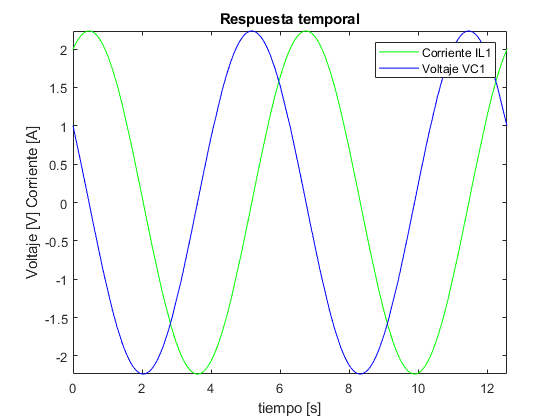
\includegraphics[width=\maxwidth{56.196688409433015em}]{figure_0_00}
	\end{center}
	
	
	\begin{matlabcode}
		fplot(iSol,vSol)
		title('Phase Portrait')
		xlabel('Corriente [A]')
		ylabel('Voltaje [V]')
		hold off
	\end{matlabcode}
	\begin{center}
		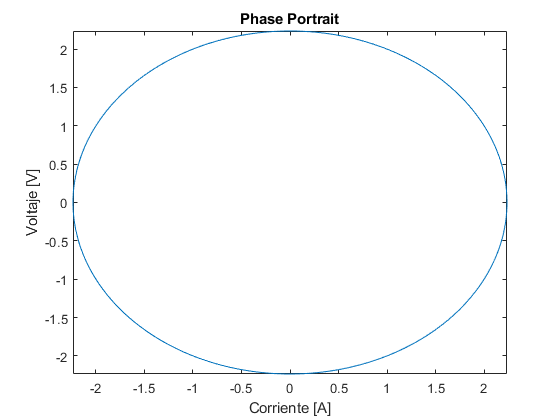
\includegraphics[width=\maxwidth{56.196688409433015em}]{figure_1_00}
	\end{center}
	
	\subsection{Ejercicio 2} Mostrar que los valores propios del circuito de la Figura \ref{fig2} son $-1\pm j$. Encontrar la solución completa para condiciones iniciales arbitrarias y una excitación arbitraria $E(t)$. Sea $C=1F$, $L=1H$, $R_1=R_2=1\Omega$. Graficar la trayectoria de la solución homogénea para dos condiciones iniciales en el espacio de estados.\\
	 \begin{center}
		\begin{circuitikz}[american voltages]\label{fig2}
			\ctikzset{label/align = smart}
			\draw (0,0) node[ground]{} 
			(0,0) to [V,label=E(t)](0,2)
			(0,2) to [R, label=$R_1$]++(2,0) to [short,-*]++(0,0) coordinate (nodo1) to [C,l=C]++(0,-2) node[ground]{}
			(nodo1) to [L,label=L]++(2,0) to [R,l=$R_2$]++(0,-2) node[ground]{}
			;
		\end{circuitikz}
	\\ Figura \ref{fig2}
	\end{center}
\begin{par}
	\begin{flushleft}
		Se definen simbólicas las variables
	\end{flushleft}
\end{par}

\begin{matlabcode}
	syms t vc(t) il(t) C L R1 R2 E;
\end{matlabcode}

\begin{par}
	\begin{flushleft}
		Se plantean las ecuaciones y se obtienen las matrices de la forma generalizada
	\end{flushleft}
\end{par}

\begin{matlabcode}
	M=[-C 0;0 L]
\end{matlabcode}
\begin{matlabsymbolicoutput}
	M = 
	$\displaystyle \left(\begin{array}{cc}
	-C & 0\\
	0 & L
	\end{array}\right)$
\end{matlabsymbolicoutput}
\begin{matlabcode}
	N=[-1/R1 -1;-1 R2]
\end{matlabcode}
\begin{matlabsymbolicoutput}
	N = 
	$\displaystyle \left(\begin{array}{cc}
	-\frac{1}{R_1 } & -1\\
	-1 & R_2 
	\end{array}\right)$
\end{matlabsymbolicoutput}
\begin{matlabcode}
	u=[-E/R1;0]
\end{matlabcode}
\begin{matlabsymbolicoutput}
	u = 
	$\displaystyle \left(\begin{array}{c}
	-\frac{\textrm{E}}{R_1 }\\
	0
	\end{array}\right)$
\end{matlabsymbolicoutput}

\begin{par}
	\begin{flushleft}
		Se expresan las matrices de la forma normalizada
	\end{flushleft}
\end{par}

\vspace{1em}

\begin{matlabcode}
	A=-1.*(M\N)
\end{matlabcode}
\begin{matlabsymbolicoutput}
	A = 
	$\displaystyle \left(\begin{array}{cc}
	-\frac{1}{C R_1 } & -\frac{1}{C}\\
	\frac{1}{L} & -\frac{R_2 }{L}
	\end{array}\right)$
\end{matlabsymbolicoutput}
\begin{matlabcode}
	
	B=M\u
\end{matlabcode}
\begin{matlabsymbolicoutput}
	B = 
	$\displaystyle \left(\begin{array}{c}
	\frac{\textrm{E}}{C R_1 }\\
	0
	\end{array}\right)$
\end{matlabsymbolicoutput}

\begin{par}
	\begin{flushleft}
		Se definen las variables de estado
	\end{flushleft}
\end{par}

\begin{matlabcode}
	x=[vc;il]
\end{matlabcode}
\begin{matlabsymbolicoutput}
	x(t) = 
	$\displaystyle \left(\begin{array}{c}
	\textrm{vc}\left(t\right)\\
	\textrm{il}\left(t\right)
	\end{array}\right)$
\end{matlabsymbolicoutput}

\begin{par}
	\begin{flushleft}
		Expresando el sistema en forma diferencial
	\end{flushleft}
\end{par}

\begin{matlabcode}
	odes = diff(x) ==  A*x + B
\end{matlabcode}
\begin{matlabsymbolicoutput}
	odes(t) = 
	$\displaystyle \left(\begin{array}{c}
	\frac{\partial }{\partial t}\;\textrm{vc}\left(t\right)=\frac{\textrm{E}}{C R_1 }-\frac{\textrm{vc}\left(t\right)}{C R_1 }-\frac{\textrm{il}\left(t\right)}{C}\\
	\frac{\partial }{\partial t}\;\textrm{il}\left(t\right)=\frac{\textrm{vc}\left(t\right)}{L}-\frac{R_2  \textrm{il}\left(t\right)}{L}
	\end{array}\right)$
\end{matlabsymbolicoutput}

\begin{par}
	\begin{flushleft}
		Resolviendo el sistema con el comando dsolve
	\end{flushleft}
\end{par}

\begin{matlabcode}
	[vSol(t), iSol(t)] = dsolve(odes);
\end{matlabcode}

\begin{par}
	\begin{flushleft}
		\textbf{Tensión del capacitor}
	\end{flushleft}
\end{par}

\begin{matlabcode}
	vSol(t) = simplify(vSol(t))
\end{matlabcode}
\begin{matlabsymbolicoutput}
	vSol(t) = 
	$\displaystyle \begin{array}{l}
	\frac{e^{-\sigma_1 }  {\left(\textrm{E} e^{\sigma_1 } +C_{23}  R_1 +C_{23}  R_2 +C_{24}  R_1  \sigma_2 +C_{24}  R_2  \sigma_2 \right)}}{R_1 +R_2 }\\
	\mathrm{}\\
	\textrm{where}\\
	\mathrm{}\\
	\;\;\sigma_1 =\frac{t {\left(L+\sqrt{C^2  {R_1 }^2  {R_2 }^2 -4 C L {R_1 }^2 -2 C L R_1  R_2 +L^2 }+C R_1  R_2 \right)}}{2 C L R_1 }\\
	\mathrm{}\\
	\;\;\sigma_2 =e^{\frac{t \sqrt{C^2  {R_1 }^2  {R_2 }^2 -4 C L {R_1 }^2 -2 C L R_1  R_2 +L^2 }}{C L R_1 }} 
	\end{array}$
\end{matlabsymbolicoutput}

\begin{par}
	\begin{flushleft}
		\textbf{Corriente del inductor}
	\end{flushleft}
\end{par}

\begin{matlabcode}
	iSol(t) = simplify(iSol(t))
\end{matlabcode}
\begin{matlabsymbolicoutput}
	iSol(t) = 
	$\displaystyle \begin{array}{l}
	e^{-\frac{t \sigma_4 }{2 C L R_1 }}  {\left(R_2 -\frac{\sigma_4 }{2 C R_1 }\right)} {\left(C_{23} -\frac{2 C \textrm{E} L R_1  \sigma_1  e^{\sigma_5 }  \sigma_2 }{\sigma_4  \sigma_6 }\right)}+e^{-\frac{t \sigma_3 }{2 C L R_1 }}  {\left(R_2 -\frac{\sigma_3 }{2 C R_1 }\right)} {\left(C_{24} +\frac{2 C \textrm{E} L R_1  \sigma_1  e^{-\sigma_5 }  \sigma_2 }{\sigma_3  \sigma_6 }\right)}\\
	\mathrm{}\\
	\textrm{where}\\
	\mathrm{}\\
	\;\;\sigma_1 =e^{\frac{R_2  t}{2 L}} \\
	\mathrm{}\\
	\;\;\sigma_2 =e^{\frac{t}{2 C R_1 }} \\
	\mathrm{}\\
	\;\;\sigma_3 =L-\sigma_6 +C R_1  R_2 \\
	\mathrm{}\\
	\;\;\sigma_4 =L+\sigma_6 +C R_1  R_2 \\
	\mathrm{}\\
	\;\;\sigma_5 =\frac{t \sigma_6 }{2 C L R_1 }\\
	\mathrm{}\\
	\;\;\sigma_6 =\sqrt{C^2  {R_1 }^2  {R_2 }^2 -4 C L {R_1 }^2 -2 C L R_1  R_2 +L^2 }
	\end{array}$
\end{matlabsymbolicoutput}

\begin{par}
	\begin{flushleft}
		Reemplazando los valores de E,R1, R2, L y C
	\end{flushleft}
\end{par}

\begin{matlabcode}
	clear C L R1 R2 E;
	syms C1 C2;
	R1=1;R2=1;L=1;C=1;E=1;
	A=subs(A);
	B=subs(B);
\end{matlabcode}

\matlabheading{Autovalores del circuito}

\begin{matlabcode}
	autovalores= eig(A)
\end{matlabcode}
\begin{matlabsymbolicoutput}
	autovalores = 
	$\displaystyle \left(\begin{array}{c}
	-1-i\\
	-1+i
	\end{array}\right)$
\end{matlabsymbolicoutput}

\begin{par}
	\begin{flushleft}
		Las ecuaciones diferenciales son
	\end{flushleft}
\end{par}

\begin{matlabcode}
	odes = diff(x) == A*x + B
\end{matlabcode}
\begin{matlabsymbolicoutput}
	odes(t) = 
	$\displaystyle \left(\begin{array}{c}
	\frac{\partial }{\partial t}\;\textrm{vc}\left(t\right)=1-\textrm{vc}\left(t\right)-\textrm{il}\left(t\right)\\
	\frac{\partial }{\partial t}\;\textrm{il}\left(t\right)=\textrm{vc}\left(t\right)-\textrm{il}\left(t\right)
	\end{array}\right)$
\end{matlabsymbolicoutput}

\matlabheading{Estableciendo condiciones iniciales y tiempo de simulación}

\begin{par}
	\begin{flushleft}
		Para el primer par de condiciones iniciales
	\end{flushleft}
\end{par}

\begin{matlabcode}
	v0=1;
	i0=1;
	ti=0;
	tf=4*pi;
	Xant=[v0;i0];
	constantes=x(0)==Xant;
	[vSol(t), iSol(t)] = dsolve(odes,constantes)
\end{matlabcode}
\begin{matlabsymbolicoutput}
	vSol(t) = 
	$\displaystyle \frac{e^{-t}  \cos \left(t\right)}{2}+\frac{e^{-t}  \sin \left(t\right)}{2}+\frac{1}{2}$
	iSol(t) = 
	$\displaystyle \frac{e^{-t}  \cos \left(t\right)}{2}-\frac{e^{-t}  \sin \left(t\right)}{2}+\frac{1}{2}$
\end{matlabsymbolicoutput}


\begin{par}
	\begin{flushleft}
		Para el segundo par de condiciones iniciales
	\end{flushleft}
\end{par}

\begin{matlabcode}
	clear t;
	syms t;
	v0=-1;
	i0=-1;
	ti=0;
	tf=4*pi;
	Xant=[v0;i0];
	constantes=x(0)==Xant;
	[v2Sol(t), i2Sol(t)] = dsolve(odes,constantes)
\end{matlabcode}
\begin{matlabsymbolicoutput}
	v2Sol(t) = 
	$\displaystyle \frac{1}{2}-\frac{3 e^{-t}  \sin \left(t\right)}{2}-\frac{3 e^{-t}  \cos \left(t\right)}{2}$
	i2Sol(t) = 
	$\displaystyle \frac{3 e^{-t}  \sin \left(t\right)}{2}-\frac{3 e^{-t}  \cos \left(t\right)}{2}+\frac{1}{2}$
\end{matlabsymbolicoutput}

\begin{par}
	\begin{flushleft}
		Gráfico de las soluciones
	\end{flushleft}
\end{par}

\begin{matlabcode}
	h=0.1;
	t=ti:h:tf;
	b=plot(i2Sol(t),v2Sol(t),'-b',iSol(t),vSol(t),'-r');
	title('Phase portrait')
	xlabel('Corriente en el inductor [A]')
	ylabel('Voltaje en el capacitor [V]')
	grid on
	legend({'[vo=1;io=10]','[vo=1;i0=1]'})
	xlim([-1.00 1.00])
	ylim([-1.00 1.00])
\end{matlabcode}
\begin{center}
	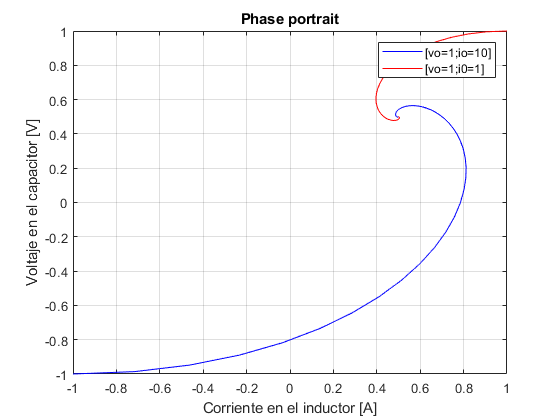
\includegraphics[width=\maxwidth{56.196688409433015em}]{figure_0_01}
\end{center}
	
	\subsection{Ejercicio 3} Para el circuito de la Figura \ref{fig3}, $C_1=C_2=C_3=1F$, $R_1=R_2=1\Omega$. Mostrar que los valores propios son $-1$ y $-\frac{1}{3}$. Asumir que la excitacion $E(t)=10\cos(\omega t)$. Encontrar la respuesta de estado estacionario.
	\begin{center}
		\begin{circuitikz}[american voltages]\label{fig3}
			\ctikzset{label/align = smart}
			\draw (0,0) node[ground]{} 
			(0,0) to [V,label=E(t)](0,2)
			(0,2) to [R, label=$R_1$]++(2,0) to [short,-*]++(0,0) coordinate (nodo1) to [C,l=$C_1$]++(0,-2) node[ground]{}
			(nodo1) to [C,label=$C_3$]++(2,0) to [short,-*]++(0,0) coordinate (nodo2) to [C,l=$C_2$]++(0,-2) node[ground]{}
			(nodo2) to [short]++(2,0) to [R,label=$R_2$]++(0,-2) node[ground]{}
			;
		\end{circuitikz}
		\\ Figura \ref{fig3}
	\end{center}

\begin{par}
	\begin{flushleft}
		Se definen simbólicas las variables
	\end{flushleft}
\end{par}

\begin{matlabcode}
	syms t vc1(t) vc2(t) C1 C2 C3 R1 R2 w;
\end{matlabcode}

\begin{par}
	\begin{flushleft}
		Se plantean las ecuaciones y se obtienen las matrices de la forma generalizada
	\end{flushleft}
\end{par}

\begin{matlabcode}
	M=[C3 -C2;C1+C3 C1]
\end{matlabcode}
\begin{matlabsymbolicoutput}
	M = 
	$\displaystyle \left(\begin{array}{cc}
	C_3  & -C_2 \\
	C_1 +C_3  & C_1 
	\end{array}\right)$
\end{matlabsymbolicoutput}
\begin{matlabcode}
	N=[0 -1/R2; 1/R1 1/R1]
\end{matlabcode}
\begin{matlabsymbolicoutput}
	N = 
	$\displaystyle \left(\begin{array}{cc}
	0 & -\frac{1}{R_2 }\\
	\frac{1}{R_1 } & \frac{1}{R_1 }
	\end{array}\right)$
\end{matlabsymbolicoutput}
\begin{matlabcode}
	u=[0;10*cos(w*t)/R1];
\end{matlabcode}

\begin{par}
	\begin{flushleft}
		Se expresan las matrices de la forma normalizada
	\end{flushleft}
\end{par}

\begin{matlabcode}
	A=-1.*(M\N)
\end{matlabcode}
\begin{matlabsymbolicoutput}
	A = 
	$\displaystyle \begin{array}{l}
	\left(\begin{array}{cc}
	-\frac{C_2 }{\sigma_2 } & \frac{C_1  R_1 -C_2  R_2 }{\sigma_1 }\\
	-\frac{C_3 }{\sigma_2 } & -\frac{C_1  R_1 +C_3  R_1 +C_3  R_2 }{\sigma_1 }
	\end{array}\right)\\
	\mathrm{}\\
	\textrm{where}\\
	\mathrm{}\\
	\;\;\sigma_1 =R_1  R_2  {\left(C_1  C_2 +C_1  C_3 +C_2  C_3 \right)}\\
	\mathrm{}\\
	\;\;\sigma_2 =R_1  {\left(C_1  C_2 +C_1  C_3 +C_2  C_3 \right)}
	\end{array}$
\end{matlabsymbolicoutput}
\begin{matlabcode}
	
	B=M\u
\end{matlabcode}
\begin{matlabsymbolicoutput}
	B = 
	$\displaystyle \left(\begin{array}{c}
	\frac{10 C_2  \cos \left(t w\right)}{R_1  {\left(C_1  C_2 +C_1  C_3 +C_2  C_3 \right)}}\\
	\frac{10 C_3  \cos \left(t w\right)}{R_1  {\left(C_1  C_2 +C_1  C_3 +C_2  C_3 \right)}}
	\end{array}\right)$
\end{matlabsymbolicoutput}

\begin{par}
	\begin{flushleft}
		Se definen las variables de estado
	\end{flushleft}
\end{par}

\begin{matlabcode}
	x=[vc1;vc2]
\end{matlabcode}
\begin{matlabsymbolicoutput}
	x(t) = 
	$\displaystyle \left(\begin{array}{c}
	{\textrm{vc}}_1 \left(t\right)\\
	{\textrm{vc}}_2 \left(t\right)
	\end{array}\right)$
\end{matlabsymbolicoutput}

\begin{par}
	\begin{flushleft}
		Expresando el sistema en forma diferencial
	\end{flushleft}
\end{par}

\begin{matlabcode}
	odes = diff(x) ==  A*x + B
\end{matlabcode}
\begin{matlabsymbolicoutput}
	odes(t) = 
	$\displaystyle \begin{array}{l}
	\left(\begin{array}{c}
	\frac{\partial }{\partial t}\;{\textrm{vc}}_1 \left(t\right)=\frac{10 C_2  \cos \left(t w\right)}{R_1  \sigma_1 }-\frac{C_2  {\textrm{vc}}_1 \left(t\right)}{R_1  \sigma_1 }+\frac{{\textrm{vc}}_2 \left(t\right) {\left(C_1  R_1 -C_2  R_2 \right)}}{R_1  R_2  \sigma_1 }\\
	\frac{\partial }{\partial t}\;{\textrm{vc}}_2 \left(t\right)=\frac{10 C_3  \cos \left(t w\right)}{R_1  \sigma_1 }-\frac{C_3  {\textrm{vc}}_1 \left(t\right)}{R_1  \sigma_1 }-\frac{{\textrm{vc}}_2 \left(t\right) {\left(C_1  R_1 +C_3  R_1 +C_3  R_2 \right)}}{R_1  R_2  \sigma_1 }
	\end{array}\right)\\
	\mathrm{}\\
	\textrm{where}\\
	\mathrm{}\\
	\;\;\sigma_1 =C_1  C_2 +C_1  C_3 +C_2  C_3 
	\end{array}$
\end{matlabsymbolicoutput}

\begin{par}
	\begin{flushleft}
		Reemplazando los valores de R1, R2 y los capacitores
	\end{flushleft}
\end{par}

\begin{matlabcode}
	clear C1 C2 C3 R1 R2 w;
	syms C11 C12;
	R1=1;R2=1;C1=1;C2=1;C3=1;w=1;
	A=subs(A);
	B=subs(B);
\end{matlabcode}

\matlabheading{Autovalores del circuito}

\begin{matlabcode}
	autovalores= eig(A)
\end{matlabcode}
\begin{matlabsymbolicoutput}
	autovalores = 
	$\displaystyle \left(\begin{array}{c}
	-1\\
	-\frac{1}{3}
	\end{array}\right)$
\end{matlabsymbolicoutput}

\begin{par}
	\begin{flushleft}
		Las ecuaciones diferenciales son
	\end{flushleft}
\end{par}

\begin{matlabcode}
	odes = diff(x) == A*x + B
\end{matlabcode}
\begin{matlabsymbolicoutput}
	odes(t) = 
	$\displaystyle \left(\begin{array}{c}
	\frac{\partial }{\partial t}\;{\textrm{vc}}_1 \left(t\right)=\frac{10 \cos \left(t\right)}{3}-\frac{{\textrm{vc}}_1 \left(t\right)}{3}\\
	\frac{\partial }{\partial t}\;{\textrm{vc}}_2 \left(t\right)=\frac{10 \cos \left(t\right)}{3}-\frac{{\textrm{vc}}_1 \left(t\right)}{3}-{\textrm{vc}}_2 \left(t\right)
	\end{array}\right)$
\end{matlabsymbolicoutput}

\matlabheading{Estableciendo condiciones iniciales y tiempo de simulación}

\begin{par}
	\begin{flushleft}
		Para el primer par de condiciones iniciales
	\end{flushleft}
\end{par}

\begin{matlabcode}
	vc01=0;
	vc02=0;
	ti=0;
	tf=6*pi;
	Xant=[vc01;vc02];
	constantes=x(0)==Xant;
	[vc1Sol(t), vc2Sol(t)] = dsolve(odes,constantes)
\end{matlabcode}
\begin{matlabsymbolicoutput}
	vc1Sol(t) = 
	$\displaystyle \sqrt{10} \cos \left(t-\textrm{atan}\left(3\right)\right)-\frac{1}{{{\left(e^t \right)}}^{1/3} }$
	vc2Sol(t) = 
	$\displaystyle \frac{1}{2 {{\left(e^t \right)}}^{1/3} }-\frac{5 e^{-t} }{2}+\sqrt{5} \cos \left(t-\textrm{atan}\left(\frac{1}{2}\right)\right)$
\end{matlabsymbolicoutput}

\begin{par}
	\begin{flushleft}
		Las exponenciales se extinguen pasado cierto tiempo y la respuesta de estado estacionario es:
	\end{flushleft}
\end{par}

\begin{par}
	$$VC_1(t)=\sqrt{10}\cos(t-\arctan{3})$$
\end{par}

\begin{par}
	$$VC_2(t)=\sqrt{5}\cos(t-\arctan{\frac{1}{2}})$$
\end{par}



	\subsection{Ejercicio 4} En el circuito de la figura \ref{fig4}, sea $v_{out}(t)$ el voltaje a traves de la resistencia $R_2$ y $E(t)=2e^-2t$ para $t\geq 0$ y $E(t)=0$ caso contrario. Mostrar que:\\
	
	
	\begin{align}
		v_{out}(t)= \left\{ \begin{array}{lcc}
		e^{-t}-\dfrac{8}{9}e^{-t}-\dfrac{1}{9}e^{-\frac{1}{5}t} &   si  & t \geq 0 \\
		\\ 0 &   & otros\ casos.
		\end{array}
		\right.
	\end{align}
	
	\begin{center}
		\begin{circuitikz}[american voltages]\label{fig4}
			\ctikzset{label/align = smart}
			\draw (0,0) node[ground]{} 
			(0,0) to [V,label=E(t)](0,2)
			(0,2) to [R, label=$R_1$]++(2,0) to [L,label=$L1$]++(2,0) to [short,-*]++(0,0) coordinate (nodo1) to [L,l=$L_3$]++(0,-2) node[ground]{}
			(nodo1) to [L,label=$L2$]++(2,0) to [R,l=$R_2$]++(0,-2) node[ground]{}
			;
		\end{circuitikz}
		\\ Figura \ref{fig4}
		\end{center}
	
	\begin{par}
		\begin{flushleft}
			Se definen simbólicas las variables
		\end{flushleft}
	\end{par}
	
	\begin{matlabcode}
		syms t il1(t) il2(t) il3(t) L1 L2 L3 R1 R2 E;
	\end{matlabcode}
	
	\begin{par}
		\begin{flushleft}
			Se plantean las ecuaciones y se obtienen las matrices de la forma generalizada
		\end{flushleft}
	\end{par}
	
	\begin{matlabcode}
		M=[L1 L1+L3;L2 -L3]
	\end{matlabcode}
	\begin{matlabsymbolicoutput}
		M = 
		$\displaystyle \left(\begin{array}{cc}
		L_1  & L_1 +L_3 \\
		L_2  & -L_3 
		\end{array}\right)$
	\end{matlabsymbolicoutput}
	\begin{matlabcode}
		N=[R1 R1;R2 0]
	\end{matlabcode}
	\begin{matlabsymbolicoutput}
		N = 
		$\displaystyle \left(\begin{array}{cc}
		R_1  & R_1 \\
		R_2  & 0
		\end{array}\right)$
	\end{matlabsymbolicoutput}
	\begin{matlabcode}
		u=[E;0]
	\end{matlabcode}
	\begin{matlabsymbolicoutput}
		u = 
		$\displaystyle \left(\begin{array}{c}
		\textrm{E}\\
		0
		\end{array}\right)$
	\end{matlabsymbolicoutput}
	
	\begin{par}
		\begin{flushleft}
			Se expresan las matrices de la forma normalizada
		\end{flushleft}
	\end{par}
	
	\vspace{1em}
	
	\begin{matlabcode}
		A=-1.*(M\N)
	\end{matlabcode}
	\begin{matlabsymbolicoutput}
		A = 
		$\displaystyle \left(\begin{array}{cc}
		-\frac{L_1  R_2 +L_3  R_1 +L_3  R_2 }{L_1  L_2 +L_1  L_3 +L_2  L_3 } & -\frac{L_3  R_1 }{L_1  L_2 +L_1  L_3 +L_2  L_3 }\\
		\frac{L_1  R_2 -L_2  R_1 }{L_1  L_2 +L_1  L_3 +L_2  L_3 } & -\frac{L_2  R_1 }{L_1  L_2 +L_1  L_3 +L_2  L_3 }
		\end{array}\right)$
	\end{matlabsymbolicoutput}
	\begin{matlabcode}
		
		B=M\u
	\end{matlabcode}
	\begin{matlabsymbolicoutput}
		B = 
		$\displaystyle \left(\begin{array}{c}
		\frac{\textrm{E} L_3 }{L_1  L_2 +L_1  L_3 +L_2  L_3 }\\
		\frac{\textrm{E} L_2 }{L_1  L_2 +L_1  L_3 +L_2  L_3 }
		\end{array}\right)$
	\end{matlabsymbolicoutput}
	
	\begin{par}
		\begin{flushleft}
			Se definen las variables de estado
		\end{flushleft}
	\end{par}
	
	\begin{matlabcode}
		x=[il2;il3]
	\end{matlabcode}
	\begin{matlabsymbolicoutput}
		x(t) = 
		$\displaystyle \left(\begin{array}{c}
		{\textrm{il}}_2 \left(t\right)\\
		{\textrm{il}}_3 \left(t\right)
		\end{array}\right)$
	\end{matlabsymbolicoutput}
	
	\begin{par}
		\begin{flushleft}
			Expresando el sistema en forma diferencial
		\end{flushleft}
	\end{par}
	
	\begin{matlabcode}
		odes = diff(x) ==  A*x + B
	\end{matlabcode}
	\begin{matlabsymbolicoutput}
		odes(t) = 
		$\displaystyle \begin{array}{l}
		\left(\begin{array}{c}
		\frac{\partial }{\partial t}\;{\textrm{il}}_2 \left(t\right)=\frac{\textrm{E} L_3 }{\sigma_1 }-\frac{{\textrm{il}}_2 \left(t\right) {\left(L_1  R_2 +L_3  R_1 +L_3  R_2 \right)}}{\sigma_1 }-\frac{L_3  R_1  {\textrm{il}}_3 \left(t\right)}{\sigma_1 }\\
		\frac{\partial }{\partial t}\;{\textrm{il}}_3 \left(t\right)=\frac{{\textrm{il}}_2 \left(t\right) {\left(L_1  R_2 -L_2  R_1 \right)}}{\sigma_1 }+\frac{\textrm{E} L_2 }{\sigma_1 }-\frac{L_2  R_1  {\textrm{il}}_3 \left(t\right)}{\sigma_1 }
		\end{array}\right)\\
		\mathrm{}\\
		\textrm{where}\\
		\mathrm{}\\
		\;\;\sigma_1 =L_1  L_2 +L_1  L_3 +L_2  L_3 
		\end{array}$
	\end{matlabsymbolicoutput}
	
	\begin{par}
		\begin{flushleft}
			Resolviendo el sistema con el comando dsolve
		\end{flushleft}
	\end{par}
	
	\begin{matlabcode}
		[i2Sol(t), i3Sol(t)] = dsolve(odes);
	\end{matlabcode}
	
	\begin{par}
		\begin{flushleft}
			Reemplazando los valores de E,R1, R2, L y C
		\end{flushleft}
	\end{par}
	
	\begin{matlabcode}
		clear L1 L2 L3 R1 R2 E;
		syms C1 C2;
		R1=1;R2=1;L1=1;L2=1;L3=2;
		E=2*exp(-2*t);
		A=subs(A);
		B=subs(B);
		odes = diff(x) == A*x + B;
	\end{matlabcode}
	
	\matlabheading{Estableciendo condiciones iniciales y tiempo de simulación}
	
	\begin{matlabcode}
		i0l2=0;
		i0l3=0;
		ti=0;
		tf=4*pi;
		Xant=[i0l2;i0l3];
		constantes=x(0)==Xant;
		[i2Sol(t), i3Sol(t)] = dsolve(odes,constantes);
	\end{matlabcode}
	
	\matlabheading{Voltaje en la resistencia R2}
	
	\begin{matlabcode}
		VR2=simplify(i2Sol*R2)
	\end{matlabcode}
	\begin{matlabsymbolicoutput}
		VR2(t) = 
		$\displaystyle -\frac{e^{-2 t}  {\left(e^{\frac{9 t}{5}} -9 e^t +8\right)}}{9}$
	\end{matlabsymbolicoutput}

	
	\subsection{Ejercicio 5} La fuente $E(t)$ del circuito de la figura \ref{fig5} se define como $E(t)=1V\ \forall t\leq 0$ y caso contrario $E(t)=0$. Mostrar que el valor a través de la resistencia $R_2$ para $t\geq 0$ es
	\begin{equation}
		v_2(t)=\frac{1}{2}e^{-t}+\frac{\sqrt{3}}{3}e^{-\dfrac{t}{2}}\sin \frac{\sqrt{3}}{3}t
	\end{equation}
	Los valores de los elementos son $R_1=R_2=1\Omega$,$C_1=C_2=1F$ y $L=2H$. Graficar la salida $v_2(t)$ para el intervalo de tiempo $0\leq t \leq 10s$.\\
	
	\begin{center}
		\begin{circuitikz}[american voltages]\label{fig5}
			\ctikzset{label/align = smart}
			\draw (0,0) node[ground]{} 
			(0,0) to [V,label=E(t)](0,2)
			(0,2) to [R, label=$R_1$]++(2,0) to [short,-*]++(0,0) coordinate (nodo1) to [C,l=$C_1$]++(0,-2) node[ground]{}
			(nodo1) to [C,label=$C_3$]++(2,0) to [short,-*]++(0,0) coordinate (nodo2) to [C,l=$C_2$]++(0,-2) node[ground]{}
			(nodo2) to [short]++(2,0) to [R,label=$R_2$]++(0,-2) node[ground]{}
			;
		\end{circuitikz}
		\\ Figura \ref{fig5}
	\end{center}
	
	\begin{par}
		\begin{flushleft}
			Se definen simbólicas las variables
		\end{flushleft}
	\end{par}
	
	\begin{matlabcode}
		syms t vc1(t) vc2(t) il1(t) R1 R2 L1 C1 C2;
	\end{matlabcode}
	
	\begin{par}
		\begin{flushleft}
			Se plantean las ecuaciones y se obtienen las matrices de la forma generalizada
		\end{flushleft}
	\end{par}
	
	\begin{matlabcode}
		M=[C1 0 0; 0 C2 0; 0 0 L1]
	\end{matlabcode}
	\begin{matlabsymbolicoutput}
		M = 
		$\displaystyle \left(\begin{array}{ccc}
		C_1  & 0 & 0\\
		0 & C_2  & 0\\
		0 & 0 & L_1 
		\end{array}\right)$
	\end{matlabsymbolicoutput}
	\begin{matlabcode}
		N=[1/R1 0 1; 0 1/R2 -1; -1 1 0]
	\end{matlabcode}
	\begin{matlabsymbolicoutput}
		N = 
		$\displaystyle \left(\begin{array}{ccc}
		\frac{1}{R_1 } & 0 & 1\\
		0 & \frac{1}{R_2 } & -1\\
		-1 & 1 & 0
		\end{array}\right)$
	\end{matlabsymbolicoutput}
	\begin{matlabcode}
		u=[0;0;0]; 
	\end{matlabcode}
	
	\begin{par}
		$$u=\begin{pmatrix}
		0\\0\\0
		\end{pmatrix}$$
	\end{par}
	
	\begin{par}
		\begin{flushleft}
			Se expresan las matrices de la forma normalizada
		\end{flushleft}
	\end{par}
	
	\begin{matlabcode}
		A=-1.*(M\N)
	\end{matlabcode}
	\begin{matlabsymbolicoutput}
		A = 
		$\displaystyle \left(\begin{array}{ccc}
		-\frac{1}{C_1  R_1 } & 0 & -\frac{1}{C_1 }\\
		0 & -\frac{1}{C_2  R_2 } & \frac{1}{C_2 }\\
		\frac{1}{L_1 } & -\frac{1}{L_1 } & 0
		\end{array}\right)$
	\end{matlabsymbolicoutput}
	
	\begin{par}
		\begin{flushleft}
			Se definen las variables de estado
		\end{flushleft}
	\end{par}
	
	\begin{matlabcode}
		x=[vc1;vc2;il1]
	\end{matlabcode}
	\begin{matlabsymbolicoutput}
		x(t) = 
		$\displaystyle \left(\begin{array}{c}
		{\textrm{vc}}_1 \left(t\right)\\
		{\textrm{vc}}_2 \left(t\right)\\
		{\textrm{il}}_1 \left(t\right)
		\end{array}\right)$
	\end{matlabsymbolicoutput}
	
	\begin{par}
		\begin{flushleft}
			Expresando el sistema en forma diferencial
		\end{flushleft}
	\end{par}
	
	\begin{matlabcode}
		odes = diff(x) == A*x
	\end{matlabcode}
	\begin{matlabsymbolicoutput}
		odes(t) = 
		$\displaystyle \left(\begin{array}{c}
		\frac{\partial }{\partial t}\;{\textrm{vc}}_1 \left(t\right)=-\frac{{\textrm{il}}_1 \left(t\right)}{C_1 }-\frac{{\textrm{vc}}_1 \left(t\right)}{C_1  R_1 }\\
		\frac{\partial }{\partial t}\;{\textrm{vc}}_2 \left(t\right)=\frac{{\textrm{il}}_1 \left(t\right)}{C_2 }-\frac{{\textrm{vc}}_2 \left(t\right)}{C_2  R_2 }\\
		\frac{\partial }{\partial t}\;{\textrm{il}}_1 \left(t\right)=\frac{{\textrm{vc}}_1 \left(t\right)}{L_1 }-\frac{{\textrm{vc}}_2 \left(t\right)}{L_1 }
		\end{array}\right)$
	\end{matlabsymbolicoutput}
	
	\begin{par}
		\begin{flushleft}
			Reemplazando los valores de los componentes
		\end{flushleft}
	\end{par}
	
	\begin{matlabcode}
		clear C1 C2 L1 R1 R2;
		syms C1 C2;
		R1=1;R2=1;C1=1;C2=1;L1=2;
		A=subs(A);
		odes = diff(x) == A*x;
	\end{matlabcode}
	
	\begin{par}
		\begin{flushleft}
			Definiendo las condiciones iniciales y tiempo de simulacion
		\end{flushleft}
	\end{par}
	
	\begin{matlabcode}
		vc01=1/2;
		vc02=1/2;
		il0=1/2;
		ti=0;
		tf=10;
		Xant=[vc01;vc02;il0];
		constantes=x(0)==Xant;
		[vc1Sol(t), vc2Sol(t), il1Sol(t)] = dsolve(odes,constantes);
	\end{matlabcode}
	
	\matlabtitle{Tensión sobre R2}
	
	\begin{matlabcode}
		simplify(vc2Sol(t))
	\end{matlabcode}
	\begin{matlabsymbolicoutput}
		ans = 
		$\displaystyle \frac{e^{-t} }{2}-\frac{\sqrt{3} \sin \left(\frac{\sqrt{3} t}{2}\right)}{3 \sqrt{e^t }}$
	\end{matlabsymbolicoutput}
	
	
	\matlabtitle{Respuesta temporal vR2(t)}
	
	\begin{matlabcode}
		clf;
		fplot(vc2Sol,[ti,tf],'-g')
		title('Respuesta temporal')
		xlabel('tiempo [s]')
		ylabel('Voltaje [V]')
		legend({'Voltaje R2'})
	\end{matlabcode}
	\begin{center}
		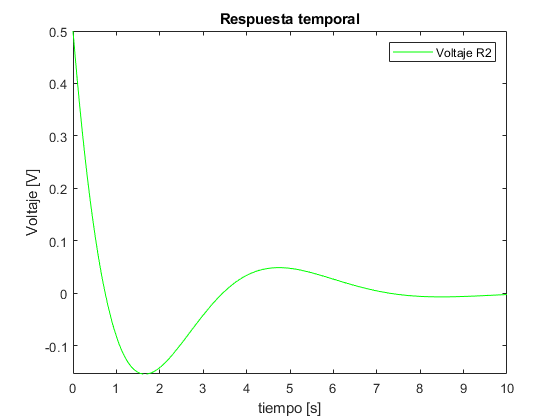
\includegraphics[width=\maxwidth{56.196688409433015em}]{figure_0_05}
	\end{center}

	
	\subsection{Ejercicio 6} Aplicar el metodo $Backward\ Euler$ para resolver las ecuaciones de estado del problema anterior siendo $E(t)=\sin t + r(t)$ dónde $r(t)$ es un ruido aleatorio cuya amplitud se encuentra uniformemente distribuida en el rango $[-0.1,0.1]$. Graficar la salida.\\
	
	\matlabheading{Valores de los componentes}
	
	\begin{matlabcode}
		R1=1;
		R2=1;
		L1=2;
		C1=1;
		C2=1;
		
		w=1;
	\end{matlabcode}
	
	\matlabheading{Condiciones iniciales}
	
	\begin{matlabcode}
		v01=0.5;
		v02=0.5;
		i01=0.5;
	\end{matlabcode}
	
	\matlabheading{Valores de tiempo y paso}
	
	\begin{matlabcode}
		ti=0;
		tf=10;
		h=0.001;
	\end{matlabcode}
	
	\matlabheading{Matrices de forma generalizadas}
	
	\begin{matlabcode}
		M=[C1 0 0;0 C2 0;0 0 L1]
	\end{matlabcode}
	\begin{matlaboutput}
		M = 3x3    
		1     0     0
		0     1     0
		0     0     2
		
	\end{matlaboutput}
	\begin{matlabcode}
		N=[1/R1 0 1;0 1/R2 -1;-1 1 0]
	\end{matlabcode}
	\begin{matlaboutput}
		N = 3x3    
		1     0     1
		0     1    -1
		-1     1     0
		
	\end{matlaboutput}
	\begin{matlabcode}
		Xant=[v01;v02;i01]
	\end{matlabcode}
	\begin{matlaboutput}
		Xant = 3x1    
		0.5000
		0.5000
		0.5000
		
	\end{matlaboutput}
	\begin{matlabcode}
		solu=[];
	\end{matlabcode}
	
	\matlabheading{Método Backward Euler}
	
	\begin{matlabcode}
		it=1;
		for i= ti:h:tf
		%Fuente variable
		E(it,1)=awgn(0.5*sin(w*i),30);
		
		%Se calcula el valor de la matriz u para cada punto 
		B=[E(it,1)/R1;0;0];
		
		X=((((1/h).*M)+N)\ B) + ((((1/h).*M)+N)\ ((1/h).*M)*Xant);
		
		solu=[solu X];
		Xant=X;
		it=it+1;
		end
		\end{matlabcode}
		
		\vspace{1em}
		
		\begin{matlabcode}
		solu=solu';
		\end{matlabcode}
		
		\matlabheading{Gráfico}
		
		\begin{matlabcode}
		t=ti:h:tf;
		plot(t,E,'-.m',t,solu(:,2),'-b')
		title('Solución respuesta temporal');
		xlabel('Tiempo [s]');
		ylabel('Tensión [V]');
		ylim([-0.7,0.7])
		grid
		\end{matlabcode}
		\begin{center}
		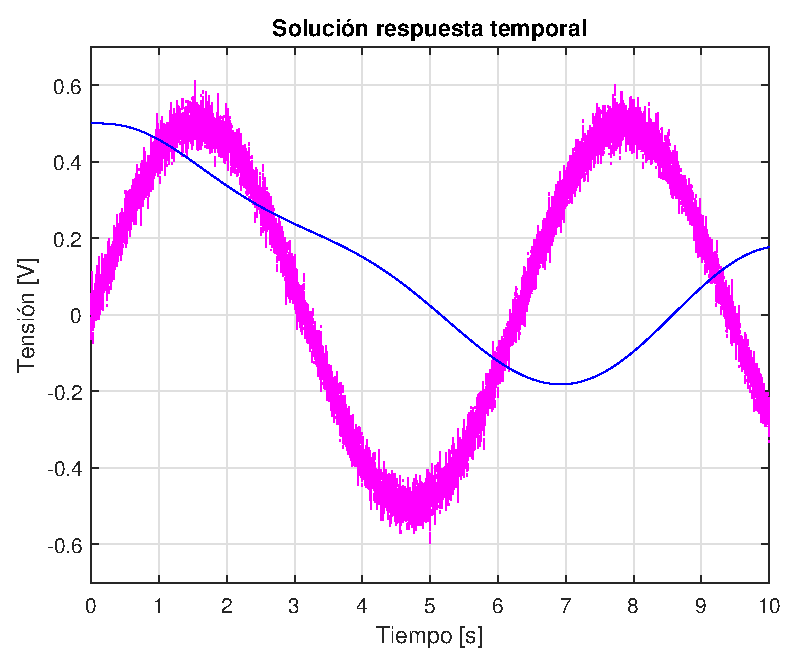
\includegraphics[width=\maxwidth{56.196688409433015em}]{figure_0_06}
		\end{center}
		
		
	\subsection{Ejercicio 7} En el circuito de la figura \ref{fig6}, suponer que el voltaje inicial del capacitor $C_1$ es $1V$, y que todas las condiciones iniciales restante son nulas. Mostrar que el voltaje a traves de $g_4$ para todo $t\geq 0$ está dado por la siguiente ecuación:
	\begin{equation}
		v_{4_n}(t)=0.225e^{\alpha t}\cos \beta t-0.0087e^{\alpha t}\sin \beta t-0.1434e^{\lambda_3 t}-0.0791e^{\lambda_4 t}
	\end{equation}
	
	Dónde $\alpha=-0.5563$, $\beta=0.9145$, $\lambda_3=-1.1255$ y $\lambda_4=-0.6786$. Los valores de los elementos son $g_1=1S$, $g_2=2S$, $g_3=3S$, $g_4=4S$, $C_1=C_2=1F$, $L_1=L_2=1H$. Graficar la proyección de la trayectoria de estado en distintos planos $2D$ para estudiar la dinámica del circuito.\\
	
	\begin{center}
		\begin{circuitikz}[american voltages]\label{fig6}
			\ctikzset{label/align = smart}
			\draw (0,0) node[ground]{} 
			(0,0) to [R,label=$g_1$](0,4)
			(0,4) to [short,-]++(2,0) coordinate (nodo1)  to [C,label=$C_1$]++(0,-2) coordinate (nodo2) to [R,label=$g_3$]++(0,-2) node[ground]{}
			(nodo1) to [short,*-]++(0,0) to [L,label=$L_1$]++(2,0) coordinate (nodo3) to [C,l=$C_2$]++(0,-2) to [R,label=$g_4$]++(0,-2) node[ground]{}
			(nodo3) to [short,*-]++(2,0) to [R,label=$g_2$]++(0,-4) node[ground]{}
			(nodo2) to [short,*-]++(0,0) to [L,label=$L_2$]++(2,0) to [short,-*]++(0,0)
			;
		\end{circuitikz}
		\\ Figura \ref{fig6}
	\end{center}
	
	
	\begin{matlabcode}
	syms t vc1(t) vc2(t) il1(t) il2(t);
	\end{matlabcode}
	
	\matlabheading{Valores de los componentes}
	
	\begin{matlabcode}
	g1=1;
	g2=2;
	g3=3;
	g4=4;
	L1=1;
	L2=1;
	C1=1;
	C2=1;
	\end{matlabcode}
	
	\begin{par}
	\begin{flushleft}
	Se plantean las ecuaciones y se obtienen las matrices de la forma generalizada
	\end{flushleft}
	\end{par}
	
	\begin{matlabcode}
	M=[C1*(1/g1 + 1/g3) 0 0 0;0 0 L1 -L2;-C1/g3 C2/g4 0 L2;0 C2*(-1/g2-1/g4) 0 0];
	N=[1 0 1/g1 -1/g3;-1 1 0 0;0 0 0 1/g4+1/g3; 0 -1 1/g2 -1/g4];
	u=[0;0;0;0];
	
	\end{matlabcode}
	
	\begin{par}
	\begin{flushleft}
	Se expresan las matrices de la forma normalizada
	\end{flushleft}
	\end{par}
	
	\begin{matlabcode}
	A=-1.*(M\N)
	\end{matlabcode}
	\begin{matlaboutput}
	A = 4x4    
	-0.7500         0   -0.7500    0.2500
	0   -1.3333    0.6667   -0.3333
	0.7500   -0.6667   -0.4167   -0.4167
	-0.2500    0.3333   -0.4167   -0.4167
	
	\end{matlaboutput}
	\begin{matlabcode}
	B=M\u
	\end{matlabcode}
	\begin{matlaboutput}
	B = 4x1    
	0
	0
	0
	0
	
	\end{matlaboutput}
	\begin{matlabcode}
	vc01=1;
	vc02=0;
	il01=0;
	il02=0;
	Xant=[vc01;vc02;il01;il02]
	\end{matlabcode}
	\begin{matlaboutput}
	Xant = 4x1    
	1
	0
	0
	0
	
	\end{matlaboutput}
	\begin{matlabcode}
	[T, lambda] = eig(A);
	syms t;
	elambda=diag(exp(eig(A).*t));
	vpa(elambda,4)
	\end{matlabcode}
	\begin{matlabsymbolicoutput}
	ans = 
	$\displaystyle \left(\begin{array}{cccc}
	e^{t {\left(-0.5563+0.9145 i\right)}}  & 0 & 0 & 0\\
	0 & e^{t {\left(-0.5563-0.9145 i\right)}}  & 0 & 0\\
	0 & 0 & e^{-1.125 t}  & 0\\
	0 & 0 & 0 & e^{-0.6786 t} 
	\end{array}\right)$
	\end{matlabsymbolicoutput}
	\begin{matlabcode}
	H=T*elambda*inv(T);
	v=H*Xant;
	\end{matlabcode}
	
	
	\begin{par}
	\begin{flushleft}
	Expresando la tensión vg4 en función de las corrientes IL2 e IC2
	\end{flushleft}
	\end{par}
	
	\begin{matlabcode}
	Ic2=C2*diff(v(2,:),t);
	Vg4=(v(4,:)+Ic2)/g4;
	vpa(Vg4,4)
	\end{matlabcode}
	\begin{matlabsymbolicoutput}
	ans = 
	\end{matlabsymbolicoutput}
	\begin{equation*}
	\begin{split}
		e^{-1.125 t}  {\left(-0.1434\right)}+e^{-0.6786 t}  {\left(-0.07908\right)}+e^{t {\left(-0.5563-0.9145 i\right)}}  {\left(0.1112-0.004343 i\right)}\\
	+e^{t {\left(-0.5563+0.9145 i\right)}}  {\left(0.1112+0.004343 i\right)}
	\end{split}
	\end{equation*}
	
	\matlabtitle{Trayectorias de estado}
	
	\begin{matlabcode}
	%Valores de los componentes
	g1=1;g2=2;g3=3;g4=4;L1=1;L2=1;C1=1;C2=1;
	%Condiciones Iniciales
	vc1=1;vc2=0;il1=0;il2=0;
	
	%Valores de tiempo y paso
	ti=0;tf=10;
	h=0.01;
	
	%Matrices del circuito 
	%Lleva la forma de:
	%M*(dx/dt)+N*x=u(t);
	
	M=[C1*(1/g1 + 1/g3) 0 0 0;0 0 L1 -L2;-C1/g3 C2/g4 0 L2;0 C2*(-1/g2-1/g4) 0 0];
	N=[1 0 1/g1 -1/g3;-1 1 0 0;0 0 0 1/g4+1/g3; 0 -1 1/g2 -1/g4];
	u=[0;0;0;0];
	
	%Condiciones iniciales
	Xant=[vc1;vc2;il1;il2];
	
	%Se lleva a la forma 
	% dx/dt=q(t)-P*x
	
	P=-1.*(M\N);
	solu=[];
	%Método RK4
	it=1;
	for i= ti:h:tf
	k1= (q+P*Xant).*h;
	Xant2=Xant+(k1.*0.5);
	k2=(q+P*Xant2).*h;
	Xant3=Xant+(k2.*0.5);
	k3=(q+P*Xant3).*h;
	Xant4=Xant+k3;
	k4=(q+P*Xant4).*h;
	X=Xant+(k1+2.*k2+2.*k3+k4)/6;
	solu=[solu X];
	Xant=X;
	it=it+1;
	end
	solu=solu';
	t=ti:h:tf;
	\end{matlabcode}
	
	
	\begin{matlabcode}
	plot(solu(:,3),solu(:,1),'-b');
	hold on 
	plot(solu(:,3),solu(:,2),'-g');
	hold on 
	plot(solu(:,4),solu(:,1),'-r');
	hold on 
	plot(solu(:,4),solu(:,2),'-m');
	hold off
	title('Phase portrait');
	xlabel('Corriente');
	ylabel('Tensión'); 
	legend({'VC1 vs iL1','VC2 vs iL1','VC1 vs iL2','VC2 vs iL2'})
	\end{matlabcode}
	\begin{center}
	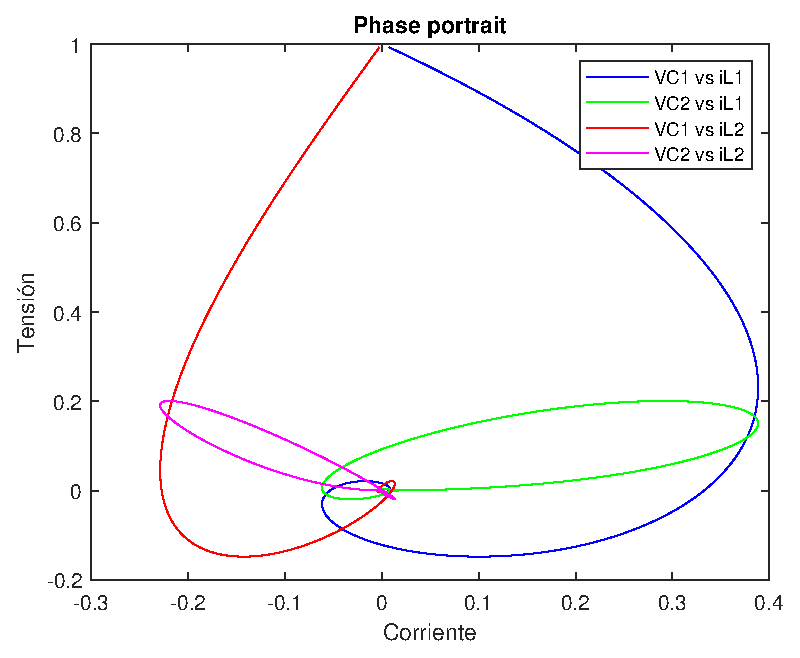
\includegraphics[width=\maxwidth{56.196688409433015em}]{figure_0_07}
	\end{center}
	
	
	\subsection{Ejercicio 8} Mostar que en el circuito de la figura \ref{fig7} el voltaje a través de $R_2$ es, con una precision de 4 dígitos:
	\begin{equation}
		v_2(t)=\int_{0}^{t}\left[0.4813e^{\lambda_1(t-\tau)}-0.0440e^{\lambda_2(t-\tau)}\right]E(\tau)d\tau
	\end{equation}
	
	Dónde $\lambda_1=-0.9645$ y $\lambda_2=-0.0882$. Asumir que todas las condiciones iniciales son cero. Sea la entrada un pulso $E(t)=\sin^2(\frac{\pi t}{5})$ para el intervalo de tiempo $0\leq t\leq 5$, $E(t)=0$ caso contrario. Encontrar el valor de $v_2(t)$ para el intervalo $0\leq t\leq 10$. Usar convolución numérica y comparar la solución con la obtenida por $Backwar\ Euler$. Los valores de los elementos son $C_1=1F$, $C_2=2F$, $C_3=3F$, $C_4=4F$, $C_5=5F$, $C_6=6F$, y $R_1=R_2=1\Omega$\\
	
	\begin{center}
		\begin{circuitikz}[american voltages]\label{fig7}
			\ctikzset{label/align = smart}
			\draw (0,0) node[ground]{} 
			(0,0) to [V,label=$E(t)$](0,4)
			(0,4) to [R,label=$R1$]++(2,0) coordinate (nodo1)  to [C,label=$C_1$]++(0,-2) coordinate (nodo2) to [C,label=$C_3$]++(0,-2) node[ground]{}
			(nodo1) to [short,*-]++(0,0) to [C,label=$C_5$]++(2,0) coordinate (nodo3) to [C,l=$C_2$]++(0,-2) to [C,label=$C_4$]++(0,-2) node[ground]{}
			(nodo3) to [short,*-]++(2,0) to [R,label=$R_2$]++(0,-4) node[ground]{}
			(nodo2) to [short,*-]++(0,0) to [C,label=$C_6$]++(2,0) to [short,-*]++(0,0)
			;
		\end{circuitikz}
		\\ Figura \ref{fig7}
	\end{center}
	
	\matlabheading{Respuesta al impulso}
	
	\begin{matlabcode}
		syms C1 C2 C3 C4 C5 C6 s R1 R2 E1 v1 v2 v3 v4;
	\end{matlabcode}
	
	\begin{par}
		\begin{flushleft}
			La matriz de admitancias
		\end{flushleft}
	\end{par}
	
	\begin{matlabcode}
		Y=[1/R1+s*C1+s*C5 -s*C5 -s*C1 0; -s*C5 s*C5+s*C2+1/R2 0 -s*C2;-s*C1 0 s*C1+s*C3+s*C6 -s*C6;0 -s*C2 -s*C6 s*C6+s*C4+s*C2]
	\end{matlabcode}
	\begin{matlabsymbolicoutput}
		Y = 
		$\displaystyle \left(\begin{array}{cccc}
		C_1  s+C_5  s+\frac{1}{R_1 } & -C_5  s & -C_1  s & 0\\
		-C_5  s & C_2  s+C_5  s+\frac{1}{R_2 } & 0 & -C_2  s\\
		-C_1  s & 0 & C_1  s+C_3  s+C_6  s & -C_6  s\\
		0 & -C_2  s & -C_6  s & C_2  s+C_4  s+C_6  s
		\end{array}\right)$
	\end{matlabsymbolicoutput}
	\begin{matlabcode}
		Is=[E1/R1;0;0;0]
	\end{matlabcode}
	\begin{matlabsymbolicoutput}
		Is = 
		$\displaystyle \left(\begin{array}{c}
		\frac{E_1 }{R_1 }\\
		0\\
		0\\
		0
		\end{array}\right)$
	\end{matlabsymbolicoutput}
	\begin{matlabcode}
		x=[v1;v2;v3;v4];
		Y\ (Is)==x;
		eqs=Y*x==Is;
		solu=solve(eqs);
		\end{matlabcode}
		
		
		\begin{par}
		\begin{flushleft}
		Reemplazando los valores del circuito
		\end{flushleft}
		\end{par}
		
		\begin{matlabcode}
		C1=1;C2=2;C3=3;C4=4;C5=5;C6=6;R1=1;R2=1;E1=1;
		\end{matlabcode}
		
		\begin{par}
		\begin{flushleft}
		La función de transferencia $ H(s)=V2(s)/E(s)$
		\end{flushleft}
		\end{par}
		
		\begin{matlabcode}
		v2s=subs(solu.v2)
		\end{matlabcode}
		\begin{matlabsymbolicoutput}
		v2s = 
		$\displaystyle \frac{432 s}{988 s^2 +1040 s+84}$
		\end{matlabsymbolicoutput}
		
		\begin{par}
		\begin{flushleft}
		La respuesta al impulso es
		\end{flushleft}
		\end{par}
		
		\begin{matlabcode}
		vpa(rewrite(ilaplace(v2s),'exp'),4)
		\end{matlabcode}
		\begin{matlabsymbolicoutput}
		ans = 
		$\displaystyle 0.4372 e^{-0.5263 t}  {\left(1.101 e^{-0.4382 t} -0.1006 e^{0.4382 t} \right)}$
		\end{matlabsymbolicoutput}
		
		\begin{par}
		$$v2(t)=0.4813 e^{-0.9645t}-0.04398e^{-0.0881t}$$
		\end{par}
		
		
		\matlabheading{Solución con Backward-Euler}
		
		\begin{matlabcode}
		clear all;
		% Valores de los componentes
		R1=1;R2=1;C1=1;C2=2;C3=3;C4=4;C5=5;C6=6;
		% Matrices forma general
		M=[C1*R1 0 C5*R1 0;-R2*C2 0 (C5*R2+R2*C2) -R2*C2; C1 -C3 0 -C6;C2 -C4 -C2 C6+C4+C2];
		N=[1 1 0 0;-1 -1 1 0;0 0 0 0;0 0 0 0];
		% Matriz forma normal
		A=-1.*(M\N);
		% Condiciones iniciales
		v01=0;v02=0;v03=0;v04=0;v05=0;v06=0;
		Xant=[v01;v03;v05;v06];
		
		clear  t
		solu=[];
		ti=0;
		tf=10;
		h=0.1;
		for t=ti:h:tf
		if t<=5
		E=(sin(0.2*pi*t))^2;
		else
		E=0;
		end
		u=[E;0;0;0];
		X=((((1/h).*M)+N)\ u) + ((((1/h).*M)+N)\ ((1/h).*M)*Xant);
		solu=[solu X];
		Xant=X;
		end
		t=ti:h:tf;
		\end{matlabcode}
		
		
		\begin{matlabcode}
		vr2=solu(1,:)+solu(2,:)-solu(3,:);
		plot(t,vr2)
		hold on;
		\end{matlabcode}
		
		
		\matlabheading{Solución convolución numérica}
		
		\begin{matlabcode}
		clear all;
		syms t tau  
		E= sin(pi/5*tau)^2*(heaviside(tau)-heaviside(tau-5));
		imp=0.4813*exp(-0.9645*(t-tau))-0.0440*exp(-0.0882*(t-tau));
		v2int=int(imp*E,tau,0,t);
		fplot(v2int,[0,10])
		hold off;
		
		legend({'Euler','Convolución'})
		title('Respuesta temporal VR2')
		xlabel('tiempo [s]')
		ylabel('Voltaje [V]')
		\end{matlabcode}
		\begin{center}
		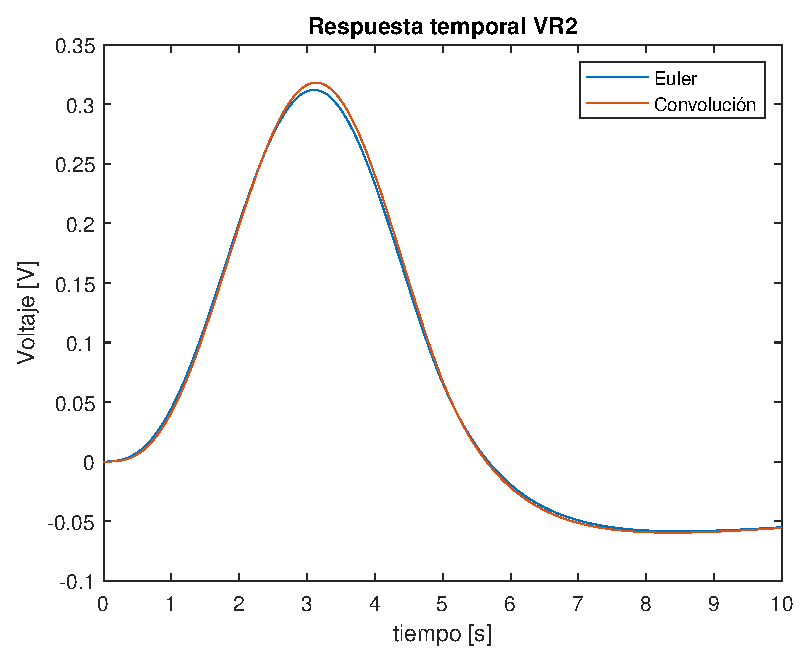
\includegraphics[width=\maxwidth{56.196688409433015em}]{figure_0_08}
		\end{center}
		
	
	\subsection{Ejercicio 9} Mostrar que la respuesta al impulso de una escalera de 5 secciones de la figura \ref{fig8}, que modela una longitud de interconexión en un circuito integrado, teniendo en cuenta que la salida es el último nodo, que $R=1\Omega$ y $C=0.1F$ y la expresión es:
	\begin{equation}
		v_{out}(t)=0.554e^{\lambda_1 t}-1.788e^{\lambda_2 t}+2.720e^{\lambda_3 t}-2.500e^{\lambda_4 t}+1.014e^{\lambda_5 t}
	\end{equation}
	
	Dónde los valores de $\lambda_n$ son los siguientes:
	\begin{center}
		\begin{tabular}{ccc}
			$\lambda_1=-36.8250$ & $\lambda_2=-28.3083$ & $\lambda_3=-17.1537$ \\ 
			$\lambda_4=-6.9028$ & $\lambda_5=-0.8101$ &  \\
		\end{tabular} 
	\end{center}

\begin{center}
	\begin{circuitikz}[american voltages]\label{fig8}
		\draw (0,0) node[ground]{}
		(0,0) to [V,label=$E(t)$](0,2)
		(0,2) to [R,label=$R_1$]++(2,0) to [short,*-]++(0,0) coordinate (nodo1) to [C,label=$C_1$]++(0,-2) node[ground]{}
		(nodo1) to [R,label=$R_2$]++(2,0) to [short,*-]++(0,0) coordinate (nodo2) to [C,label=$C_2$]++(0,-2) node[ground]{}
		(nodo2) to [R,label=$R_3$]++(2,0) to [short,*-]++(0,0) coordinate (nodo3) to [C,label=$C_3$]++(0,-2) node[ground]{}
		(nodo3) to [R,label=$R_4$]++(2,0) to [short,*-]++(0,0) coordinate (nodo4) to [C,label=$C_4$]++(0,-2) node[ground]{}
		(nodo4) to [R,label=$R_5$]++(2,0) to [C,label=$C_5$]++(0,-2) node[ground]{}
		;
	\end{circuitikz}
		\\ Figura \ref{fig8}
\end{center}

\matlabtitle{Respuesta al impulso}

\begin{matlabcode}
	syms C1 C2 C3 C4 C5 s R1 R2 R3 R4 R5 E1 v1 v2 v3 v4 v5;
\end{matlabcode}

\begin{par}
	\begin{flushleft}
		La matriz de admitancias
	\end{flushleft}
\end{par}

\begin{matlabcode}
	Y=[1/R1+s*C1+1/R2 -1/R2 0 0 0; -1/R2 1/R2+s*C2+1/R3 -1/R3 0 0;0 -1/R3 1/R3+s*C3+1/R4 -1/R4 0; 0 0 -1/R4 1/R4+s*C4+1/R5 -1/R5; 0 0 0 -1/R5 1/R5+s*C5]
\end{matlabcode}
\begin{matlabsymbolicoutput}
	Y = 
	$\displaystyle \left(\begin{array}{ccccc}
	C_1  s+\frac{1}{R_1 }+\frac{1}{R_2 } & -\frac{1}{R_2 } & 0 & 0 & 0\\
	-\frac{1}{R_2 } & C_2  s+\frac{1}{R_2 }+\frac{1}{R_3 } & -\frac{1}{R_3 } & 0 & 0\\
	0 & -\frac{1}{R_3 } & C_3  s+\frac{1}{R_3 }+\frac{1}{R_4 } & -\frac{1}{R_4 } & 0\\
	0 & 0 & -\frac{1}{R_4 } & C_4  s+\frac{1}{R_4 }+\frac{1}{R_5 } & -\frac{1}{R_5 }\\
	0 & 0 & 0 & -\frac{1}{R_5 } & C_5  s+\frac{1}{R_5 }
	\end{array}\right)$
\end{matlabsymbolicoutput}
\begin{matlabcode}
	Is=[E1/R1;0;0;0;0];
	x=[v1;v2;v3;v4;v5];
	Y\ (Is)==x;
	eqs=Y*x==Is;
	solu=solve(eqs);
	\end{matlabcode}
	
	
	\begin{par}
	\begin{flushleft}
	Reemplazando los valores del circuito
	\end{flushleft}
	\end{par}
	
	\begin{matlabcode}
	C1=0.1;C2=0.1;C3=0.1;C4=0.1;C5=0.1;R1=1;R2=1;R3=1;R4=1;R5=1;E1=1;
	\end{matlabcode}
	
	\begin{par}
	\begin{flushleft}
	La función de transferencia $ H(s)=V5(s)/E(s)$
	\end{flushleft}
	\end{par}
	
	\begin{matlabcode}
	v5s=subs(solu.v5)
	\end{matlabcode}
	\begin{matlabsymbolicoutput}
	v5s = 
	$\displaystyle \frac{1}{\frac{s^5 }{100000}+\frac{9 s^4 }{10000}+\frac{7 s^3 }{250}+\frac{7 s^2 }{20}+\frac{3 s}{2}+1}$
	\end{matlabsymbolicoutput}
	\begin{matlabcode}
	v5t=vpa(rewrite(ilaplace(v5s),'exp'),4)
	\end{matlabcode}
	\begin{matlabsymbolicoutput}
	v5t = 
	$\displaystyle 2.72 e^{-17.15 t} +0.5539 e^{-36.83 t} +1.014 e^{-0.8101 t} -2.5 e^{-6.903 t} -1.788 e^{-28.31 t} $
	\end{matlabsymbolicoutput}
	
	
	\matlabtitle{Respuesta al pulso con método Backward Euler}
	
	\begin{matlabcode}
	vc1=0;vc2=0;vc3=0;vc4=0;vc5=0;
	Xant=[vc1;vc2;vc3;vc4;vc5];
	ti=0;
	tf=10;
	h=0.01;
	M=[C1 0 0 0 0; 0 C2 0 0 0; 0 0 C3 0 0; 0 0 0 C4 0; 0 0 0 0 C5];
	N=[1/R1+1/R2 -1/R2 0 0 0; -1/R2 1/R2+1/R3 -1/R3 0 0; 0 -1/R3 1/R3+1/R4 -1/R4 0; 0 0 -1/R4 1/R4+1/R5 -1/R5; 0 0 0 -1/R5 1/R5];
	solu=[];
	it=1;
	for i= ti:h:tf
	%Fuente variable
	if i<1
	E(it,1)=1;
	else
	E(it,1)=0;
	end
	
	%Se calcula el valor de la matriz u para cada punto 
	u=[E(it,1)/R1;0;0;0;0];
	
	X=((((1/h).*M)+N)\ u) + ((((1/h).*M)+N)\ ((1/h).*M)*Xant);
	
	solu=[solu X];
	Xant=X;
	it=it+1;
	end
	t=ti:h:tf;
	clf;
	plot(t,solu(5,:),'--b')
	hold on
	fplot(v5t,[0,10],'-b')
	ylim([0,0.7])
	grid;
	legend({'Rta. Pulso','Rta. Impulso'})
	title('Respuesta temporal VC5(t)')
	xlabel('tiempo [s]')
	ylabel('Voltaje [V]')
	\end{matlabcode}
	\begin{center}
	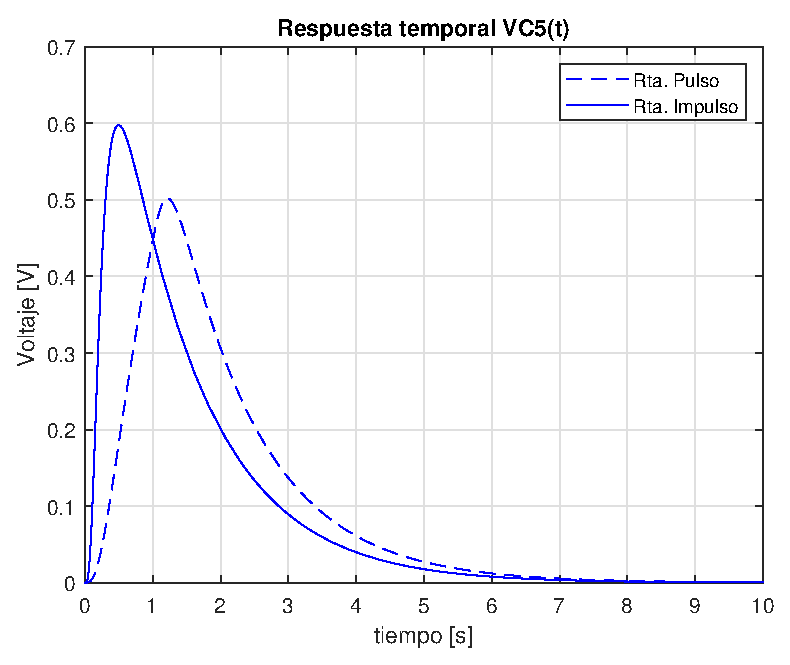
\includegraphics[width=\maxwidth{56.196688409433015em}]{figure_0_09}
	\end{center}


	\subsection{Ejercicio 10} Considerar un circuito $LC$ de cuarto orden que consiste en un inductor $L_1$ en serie con un capacitor $C_1$ y con una combinación paralelo de un inductor $L_2$ y un capacitor $C_2$. Sea $L_1=1H$, $C_1=\frac{1}{25}F$, $L_2=18H$ y $C_2=\frac{1}{72}F$. Sean las variables de estado $i_{L1}$, $i_{L2}$,$v_{C1}$, $v_{C1}$. Mostrar que las respuestas a una condición inicial $v_{C1}=1V$ son:
	\begin{center}
		\begin{tabular}{cc}
			$i_{L1}=\dfrac{-16}{165}\sin(10t)-\dfrac{1}{33}\sin(t)$& $v_{C1}=\dfrac{25}{33}\cos(t)+\dfrac{8}{33}\cos(10t)$\\
			&\\ 
			$i_{L2}=\dfrac{-4}{99}\sin(t)+\dfrac{2}{495}\sin(10t)$ & $v_{C2}=\dfrac{8}{11}\cos(10t)-\dfrac{8}{11}\cos(t)$\\
		\end{tabular} 
	\end{center}
\begin{par}
	\begin{flushleft}
		Se definen simbólicas las variables
	\end{flushleft}
\end{par}

\begin{matlabcode}
	syms t vc1(t) vc2(t) il1(t) il2(t) L1 L2 K1 K2;
\end{matlabcode}

\begin{par}
	\begin{flushleft}
		Se plantean las ecuaciones y se obtienen las matrices de la forma generalizada
	\end{flushleft}
\end{par}

\begin{matlabcode}
	M=[-K1 0 0 0;0 K2 0 0;0 0 L1 L2;0 0 0 -L2]
\end{matlabcode}
\begin{matlabsymbolicoutput}
	M = 
	$\displaystyle \left(\begin{array}{cccc}
	-K_1  & 0 & 0 & 0\\
	0 & K_2  & 0 & 0\\
	0 & 0 & L_1  & L_2 \\
	0 & 0 & 0 & -L_2 
	\end{array}\right)$
\end{matlabsymbolicoutput}
\begin{matlabcode}
	N=[0 0 1 0; 0 0 -1 1;1 0 0 0;0 1 0 0]
\end{matlabcode}
\begin{matlaboutput}
	N = 4x4    
	0     0     1     0
	0     0    -1     1
	1     0     0     0
	0     1     0     0
	
\end{matlaboutput}
\begin{matlabcode}
	u=[0;0;0;0]
\end{matlabcode}
\begin{matlaboutput}
	u = 4x1    
	0
	0
	0
	0
	
\end{matlaboutput}

\begin{par}
	\begin{flushleft}
		Se expresan las matrices de la forma normalizada
	\end{flushleft}
\end{par}

\begin{matlabcode}
	A=-1.*(M\N)
\end{matlabcode}
\begin{matlabsymbolicoutput}
	A = 
	$\displaystyle \left(\begin{array}{cccc}
	0 & 0 & \frac{1}{K_1 } & 0\\
	0 & 0 & \frac{1}{K_2 } & -\frac{1}{K_2 }\\
	-\frac{1}{L_1 } & -\frac{1}{L_1 } & 0 & 0\\
	0 & \frac{1}{L_2 } & 0 & 0
	\end{array}\right)$
\end{matlabsymbolicoutput}

\begin{par}
	\begin{flushleft}
		Se definen las variables de estado
	\end{flushleft}
\end{par}

\begin{matlabcode}
	x=[vc1;vc2;il1;il2]
\end{matlabcode}
\begin{matlabsymbolicoutput}
	x(t) = 
	$\displaystyle \left(\begin{array}{c}
	{\textrm{vc}}_1 \left(t\right)\\
	{\textrm{vc}}_2 \left(t\right)\\
	{\textrm{il}}_1 \left(t\right)\\
	{\textrm{il}}_2 \left(t\right)
	\end{array}\right)$
\end{matlabsymbolicoutput}

\begin{par}
	\begin{flushleft}
		Expresando el sistema en forma diferencial
	\end{flushleft}
\end{par}

\begin{matlabcode}
	odes = diff(x) == A*x
\end{matlabcode}
\begin{matlabsymbolicoutput}
	odes(t) = 
	$\displaystyle \left(\begin{array}{c}
	\frac{\partial }{\partial t}\;{\textrm{vc}}_1 \left(t\right)=\frac{{\textrm{il}}_1 \left(t\right)}{K_1 }\\
	\frac{\partial }{\partial t}\;{\textrm{vc}}_2 \left(t\right)=\frac{{\textrm{il}}_1 \left(t\right)}{K_2 }-\frac{{\textrm{il}}_2 \left(t\right)}{K_2 }\\
	\frac{\partial }{\partial t}\;{\textrm{il}}_1 \left(t\right)=-\frac{{\textrm{vc}}_1 \left(t\right)}{L_1 }-\frac{{\textrm{vc}}_2 \left(t\right)}{L_1 }\\
	\frac{\partial }{\partial t}\;{\textrm{il}}_2 \left(t\right)=\frac{{\textrm{vc}}_2 \left(t\right)}{L_2 }
	\end{array}\right)$
\end{matlabsymbolicoutput}

\begin{par}
	\begin{flushleft}
		Reemplazando los valores de los componentes
	\end{flushleft}
\end{par}

\begin{matlabcode}
	clear K1 K2 L1 L2;
	syms C1 C2 C3 C4;
	K1=1/25;K2=1/72;L1=1;L2=18;
	A=subs(A);
\end{matlabcode}

\begin{par}
	\begin{flushleft}
		Las ecuaciones diferenciales son
	\end{flushleft}
\end{par}

\begin{matlabcode}
	odes = diff(x) == A*x;
\end{matlabcode}

\begin{par}
	\begin{flushleft}
		Definiendo las condiciones iniciales y tiempo de simulacion
	\end{flushleft}
\end{par}

\begin{matlabcode}
	vc01=1;
	vc02=0;
	il01=0;
	il02=0;
	ti=0;
	tf=10;
	Xant=[vc01;vc02;il01;il02];
	constantes=x(0)==Xant;
	[il1Sol(t), il2Sol(t), vc1Sol(t), vc2Sol(t)] = dsolve(odes,constantes);
\end{matlabcode}


\matlabtitle{Tensión en C1}

\begin{matlabcode}
	vc1Sol
\end{matlabcode}
\begin{matlabsymbolicoutput}
	vc1Sol(t) = 
	$\displaystyle \frac{8 \cos \left(10 t\right)}{33}+\frac{25 \cos \left(t\right)}{33}$
\end{matlabsymbolicoutput}

\matlabtitle{Tensión en C2}

\begin{matlabcode}
	vc2Sol
\end{matlabcode}
\begin{matlabsymbolicoutput}
	vc2Sol(t) = 
	$\displaystyle \frac{8 \cos \left(10 t\right)}{11}-\frac{8 \cos \left(t\right)}{11}$
\end{matlabsymbolicoutput}

\matlabtitle{Corriente en L1}

\begin{matlabcode}
	il1Sol
\end{matlabcode}
\begin{matlabsymbolicoutput}
	il1Sol(t) = 
	$\displaystyle -\frac{16 \sin \left(10 t\right)}{165}-\frac{\sin \left(t\right)}{33}$
\end{matlabsymbolicoutput}

\matlabtitle{Corriente en L2}

\begin{matlabcode}
	il2Sol
\end{matlabcode}
\begin{matlabsymbolicoutput}
	il2Sol(t) = 
	$\displaystyle \frac{2 \sin \left(10 t\right)}{495}-\frac{4 \sin \left(t\right)}{99}$
\end{matlabsymbolicoutput}


\vspace{1em}

\begin{matlabcode}
	fplot(il1Sol,vc1Sol,[ti,tf])
	title('Phase Portrait')
	xlabel('iL1[A]')
	ylabel('VC1 [V]')
\end{matlabcode}
\begin{center}
	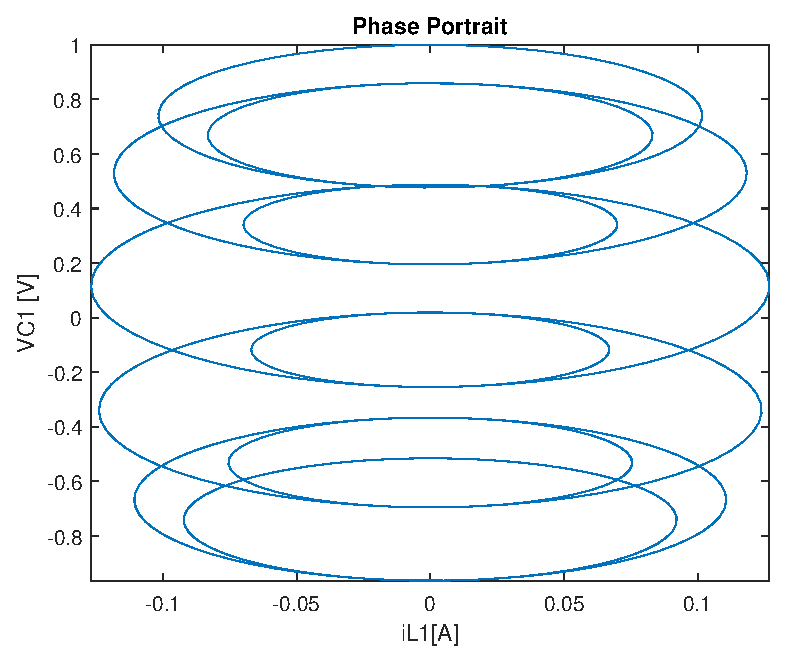
\includegraphics[width=\maxwidth{56.196688409433015em}]{figure_0_10}
\end{center}


\begin{matlabcode}
	fplot(il1Sol,vc2Sol,[ti,tf])
	title('Phase Portrait')
	xlabel('iL1[A]')
	ylabel('VC2 [V]')
\end{matlabcode}
\begin{center}
	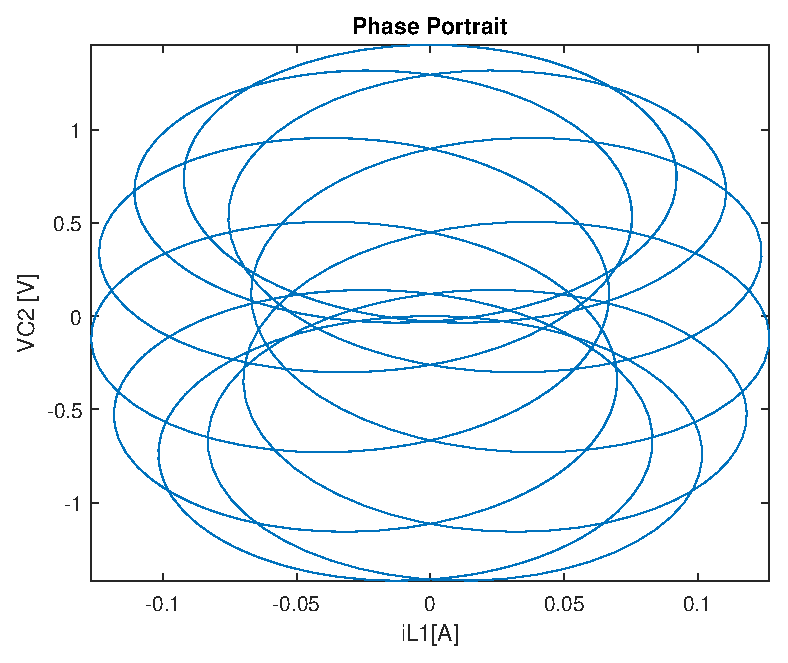
\includegraphics[width=\maxwidth{56.196688409433015em}]{figure_1_10}
\end{center}


\begin{matlabcode}
	fplot(il2Sol,vc1Sol,[ti,tf])
	title('Phase Portrait')
	xlabel('iL2[A]')
	ylabel('VC1 [V]')
\end{matlabcode}
\begin{center}
	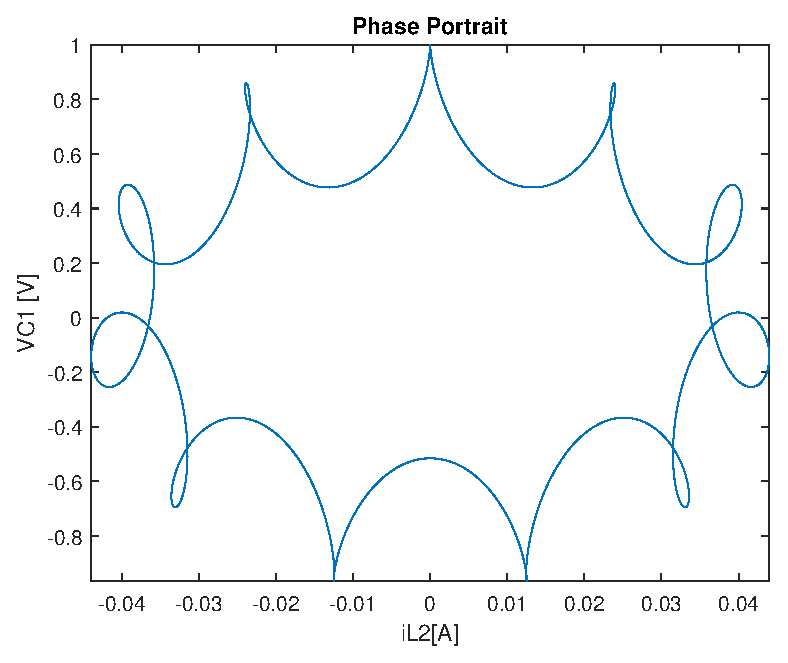
\includegraphics[width=\maxwidth{56.196688409433015em}]{figure_2_10}
\end{center}


\begin{matlabcode}
	fplot(il2Sol,vc2Sol,[ti,tf])
	title('Phase Portrait')
	xlabel('iL2[A]')
	ylabel('VC2 [V]')
\end{matlabcode}
\begin{center}
	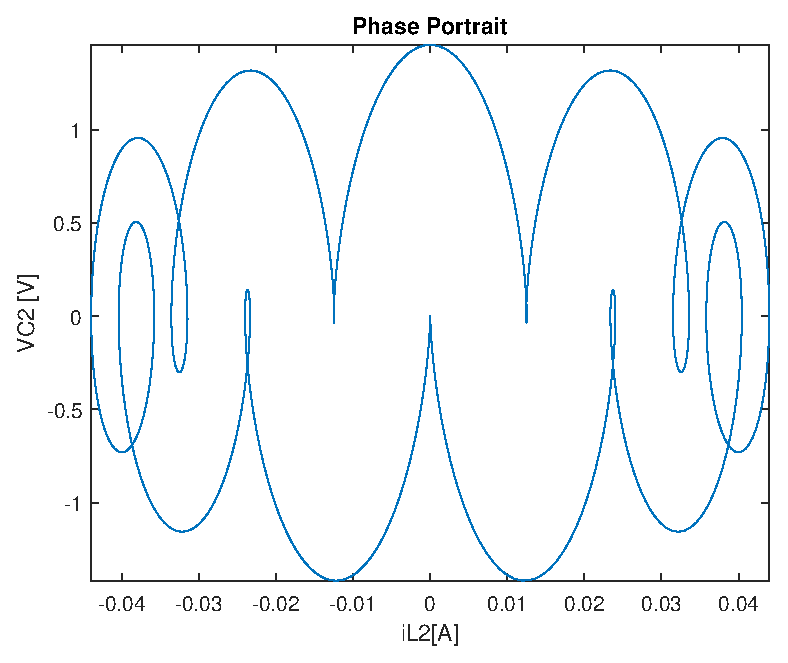
\includegraphics[width=\maxwidth{56.196688409433015em}]{figure_3_10}
\end{center}
\newpage
	\section{Conclusión}
	
	%Se encontró una herramienta muy útil para estudiar la dinámica de circuitos eléctricos que puede ser implementada de forma muy sencilla, plantear las ecuaciones de estado y obtener soluciones rápidamente. 
	%Hasta el Ejercicio 5 se utilizó un método analítico de resolución a partir de las ecuaciones de estado, desde el Ejercicio 6 se aplicaron métodos numéricos y se observó que se obtienen las soluciones con un error despreciable.\\
	
	%En el Ejercicio 8 para encontrar la respuesta temporal era necesario realizar la convolución entre la respuesta al impulso del sistema y una fuente arbitraria, para esto se desarrollaron las ecuaciones de nodos por el método de inspección y se aplicó la Transformada Inversa de Laplace, luego se comparó este resultado con la resolución a partir de variables de estado y la aplicación de un método numérico. Se observó una diferencia despreciable entre ambos métodos.\\
	
	Se aumentó la noción sobre el funcionamiento de software de simulación SPICE, ya que las ecuaciones se pueden plantear de forma sistemática y con los métodos vistos se vuelve trivial su resolución. En este trabajo se aplicaron conceptos de métodos numéricos, álgebra lineal, ecuaciones diferenciales, teoría de grafos y convolución de señales adquiridos en la carrera, lo que muestra que la Teoría de Circuitos es una rama multidisciplinaria dentro de la matemática aplicada y no solo una base para simplificar cálculos en temas más avanzados de Ingeniería Electrónica.
	
	\section{Bibliografía}
	\begin{itemize}
		\item	Wing, O. (2008). Classical circuit theory (Vol. 773). Springer Science \& Business Media.
		\item Friedland, B. (1986). Control system design: an introduction to state-space methods.
		\item Strogatz, S. (2001). Nonlinear dynamics and chaos: with applications to physics, biology, chemistry, and engineering (studies in nonlinearity).
		\item  Najm, F. N. (2010). Circuit simulation. John Wiley \& Sons.
		\item Bendtsen, C., \& Thomsen, P. G. (1999). Numerical solution of differential algebraic equations. IMM, Department of Mathematical Modelling, Technical Universityof Denmark.
		\item Zelenkov, A. A. (2011). Transient Analysis using state variables in the examples.
		\item Sander, K. F., \& Hammond, P. (1964). Linear network theory. Pergamon Press.
		\item Chapra, S. C., \& Canale, R. P. (2011). Numerical methods for engineers (Vol. 2). New York: Mcgraw-hill.
		\item Grossman, S. I., Godoy, J. J. F., \& Ernesto, D. S. A. (1983). Álgebra lineal (No. 968-422-984-4. 04-A1 LU. CG-01.). Grupo editorial iberoamericana.
	\end{itemize}
\end{document} 
